\documentclass[aspectratio=169,t,xcolor=table]{beamer}
\usepackage[utf8]{inputenc}

\usepackage{booktabs} 
\usepackage{subcaption}
\usepackage{hyperref}
\usepackage[bahasa]{babel}

\usetheme{Ufg}

\setbeamertemplate{theorems}[numbered]
\setbeamertemplate{caption}[numbered]

\definecolor{dosen}{HTML}{18426C}
\definecolor{tendik}{HTML}{F2AB1E}

%-------------------------------------------------------------%
%----------------------- Primary Definitions -----------------%

% This command set the default Color, is also possible to choose a custom color
\setPrimaryColor{UFGBlue} 

% #1 Title right #2 Vertical #3 Horizontal #4 Title left
\setLogos{lib/logos/LogoSKPB.png}{lib/logos/LogoSKPB.png}{lib/logos/M.png}{lib/logos/ITSMath.pdf}


% -------------------------------------- Title Slide Information
\begin{document}
\title[Website Kalkulus]{Perancangan Website Interaktif untuk Pembelajaran Kalkulus Menggunakan CortexJS}
\subtitle{Subdirektorat Koordinasi Perkuliahan Bersama}

\author{Teosofi Hidayah Agung}

\institute[ITS] % (optional)
{
  Institut Teknologi Sepuluh Nopember
}
\date{30 Juni 2025}
%-----------------------The next statement creates the title page.
\frame[noframenumbering]{\titlepage}


%------------------------------------------------Slide 1
\setLayout{vertical}

\begin{frame}
    \frametitle{Daftar Isi}
    \tableofcontents
\end{frame}
%---------------------------------------------------------
\section{Gambaran Umum Tempat Kerja Praktik}

\setLayout{vertical}
\subsection{Lokasi Kerja Praktik}
\begin{frame}
    \frametitle{\insertsubsection}
    \begin{columns}
        \column{0.6\textwidth}
        \begin{block}{Deskripsi Perusahaan}
            \textbf{SKPB} adalah salah satu unit kerja yang bertugas untuk mengoordinasikan perkuliahan mata kuliah bersama mahasiswa ITS, baik mahasiswa baru maupun mahasiswa lama.
        \end{block}

        \begin{alertblock}{Alamat Perusahaan}
            Gedung Menara Sains TW-1 Lt.1, Institut Teknologi Sepuluh Nopember, Surabaya.
        \end{alertblock}
    
        \begin{exampleblock}{Kegiatan Perusahaan}
            \begin{itemize}
                \item Fasilitator perkuliahan bersama.
                \item Pengawasan dan evaluasi.
                \item Pengkajian materi perkuliahan bersama.
            \end{itemize}
        \end{exampleblock}

        \column{0.4\textwidth}

            \centering
            \begin{tikzpicture}
            \node[draw=black, drop shadow, line width=1pt, inner sep=0] {
              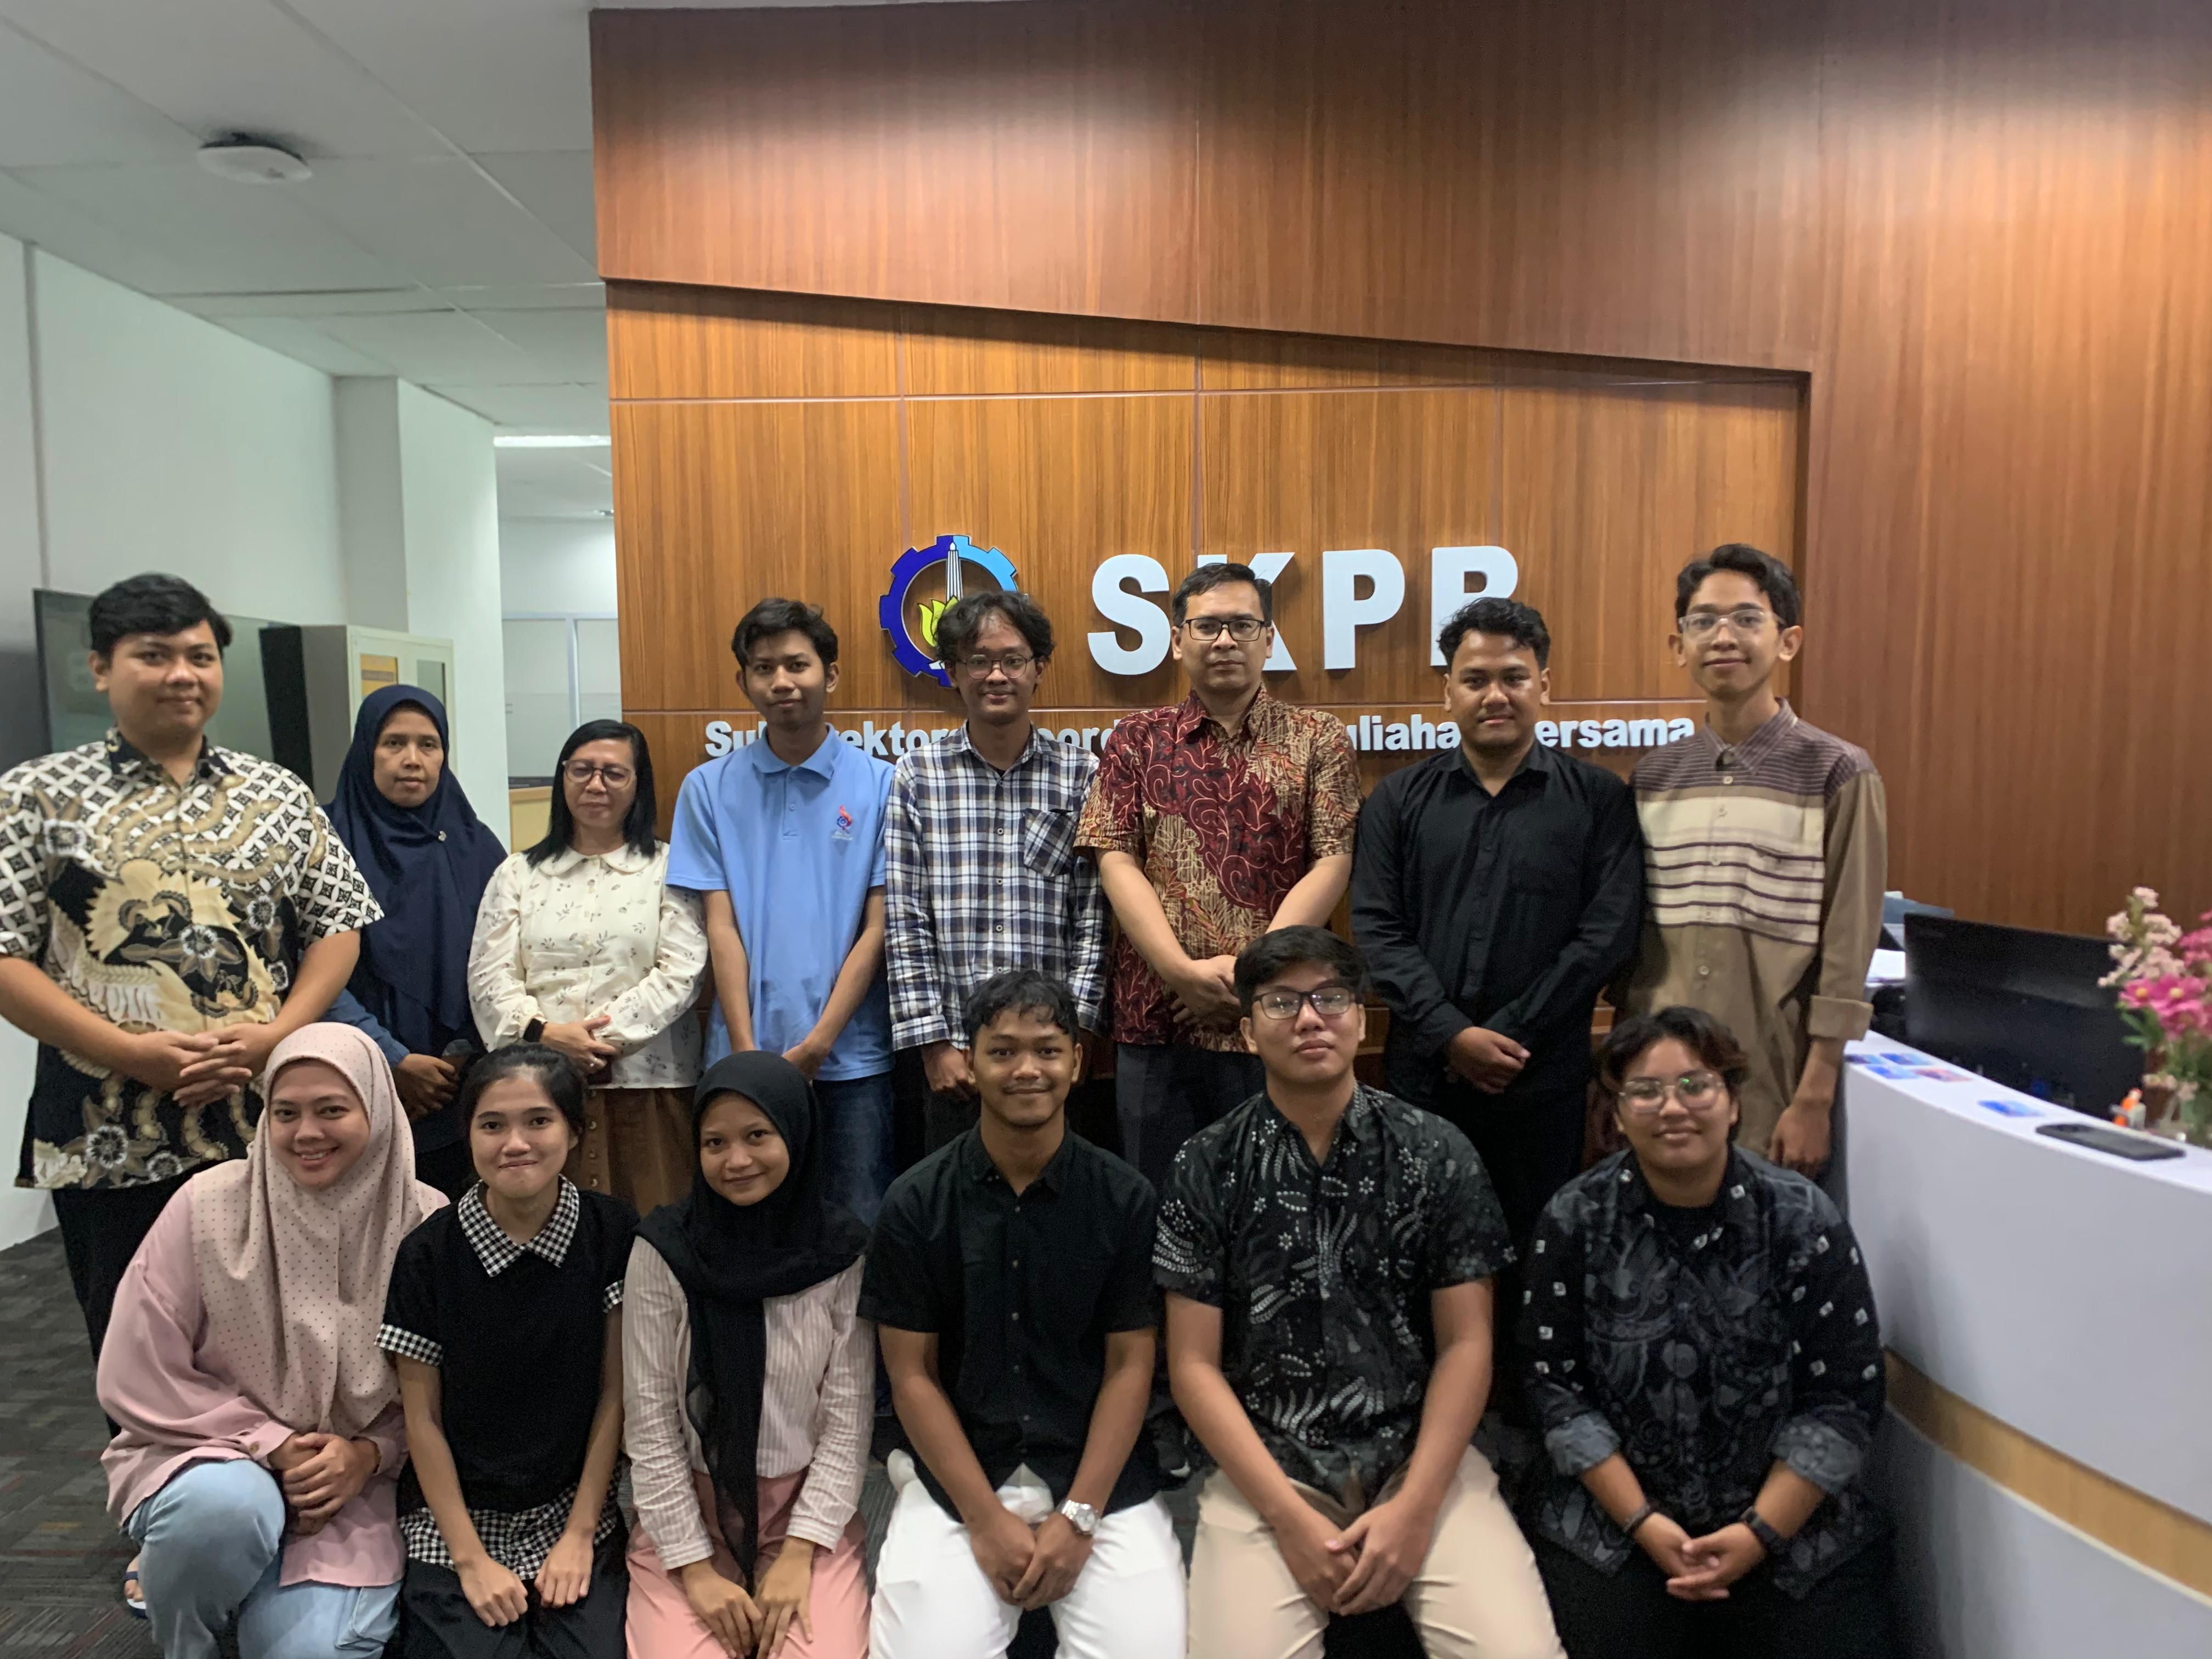
\includegraphics[width=0.8\textwidth]{figs/FotoLobbySKPB.jpg}
            };
            \end{tikzpicture}
            \\
            \begin{tikzpicture}
            \node[draw=black, drop shadow, line width=1pt, inner sep=0] {
              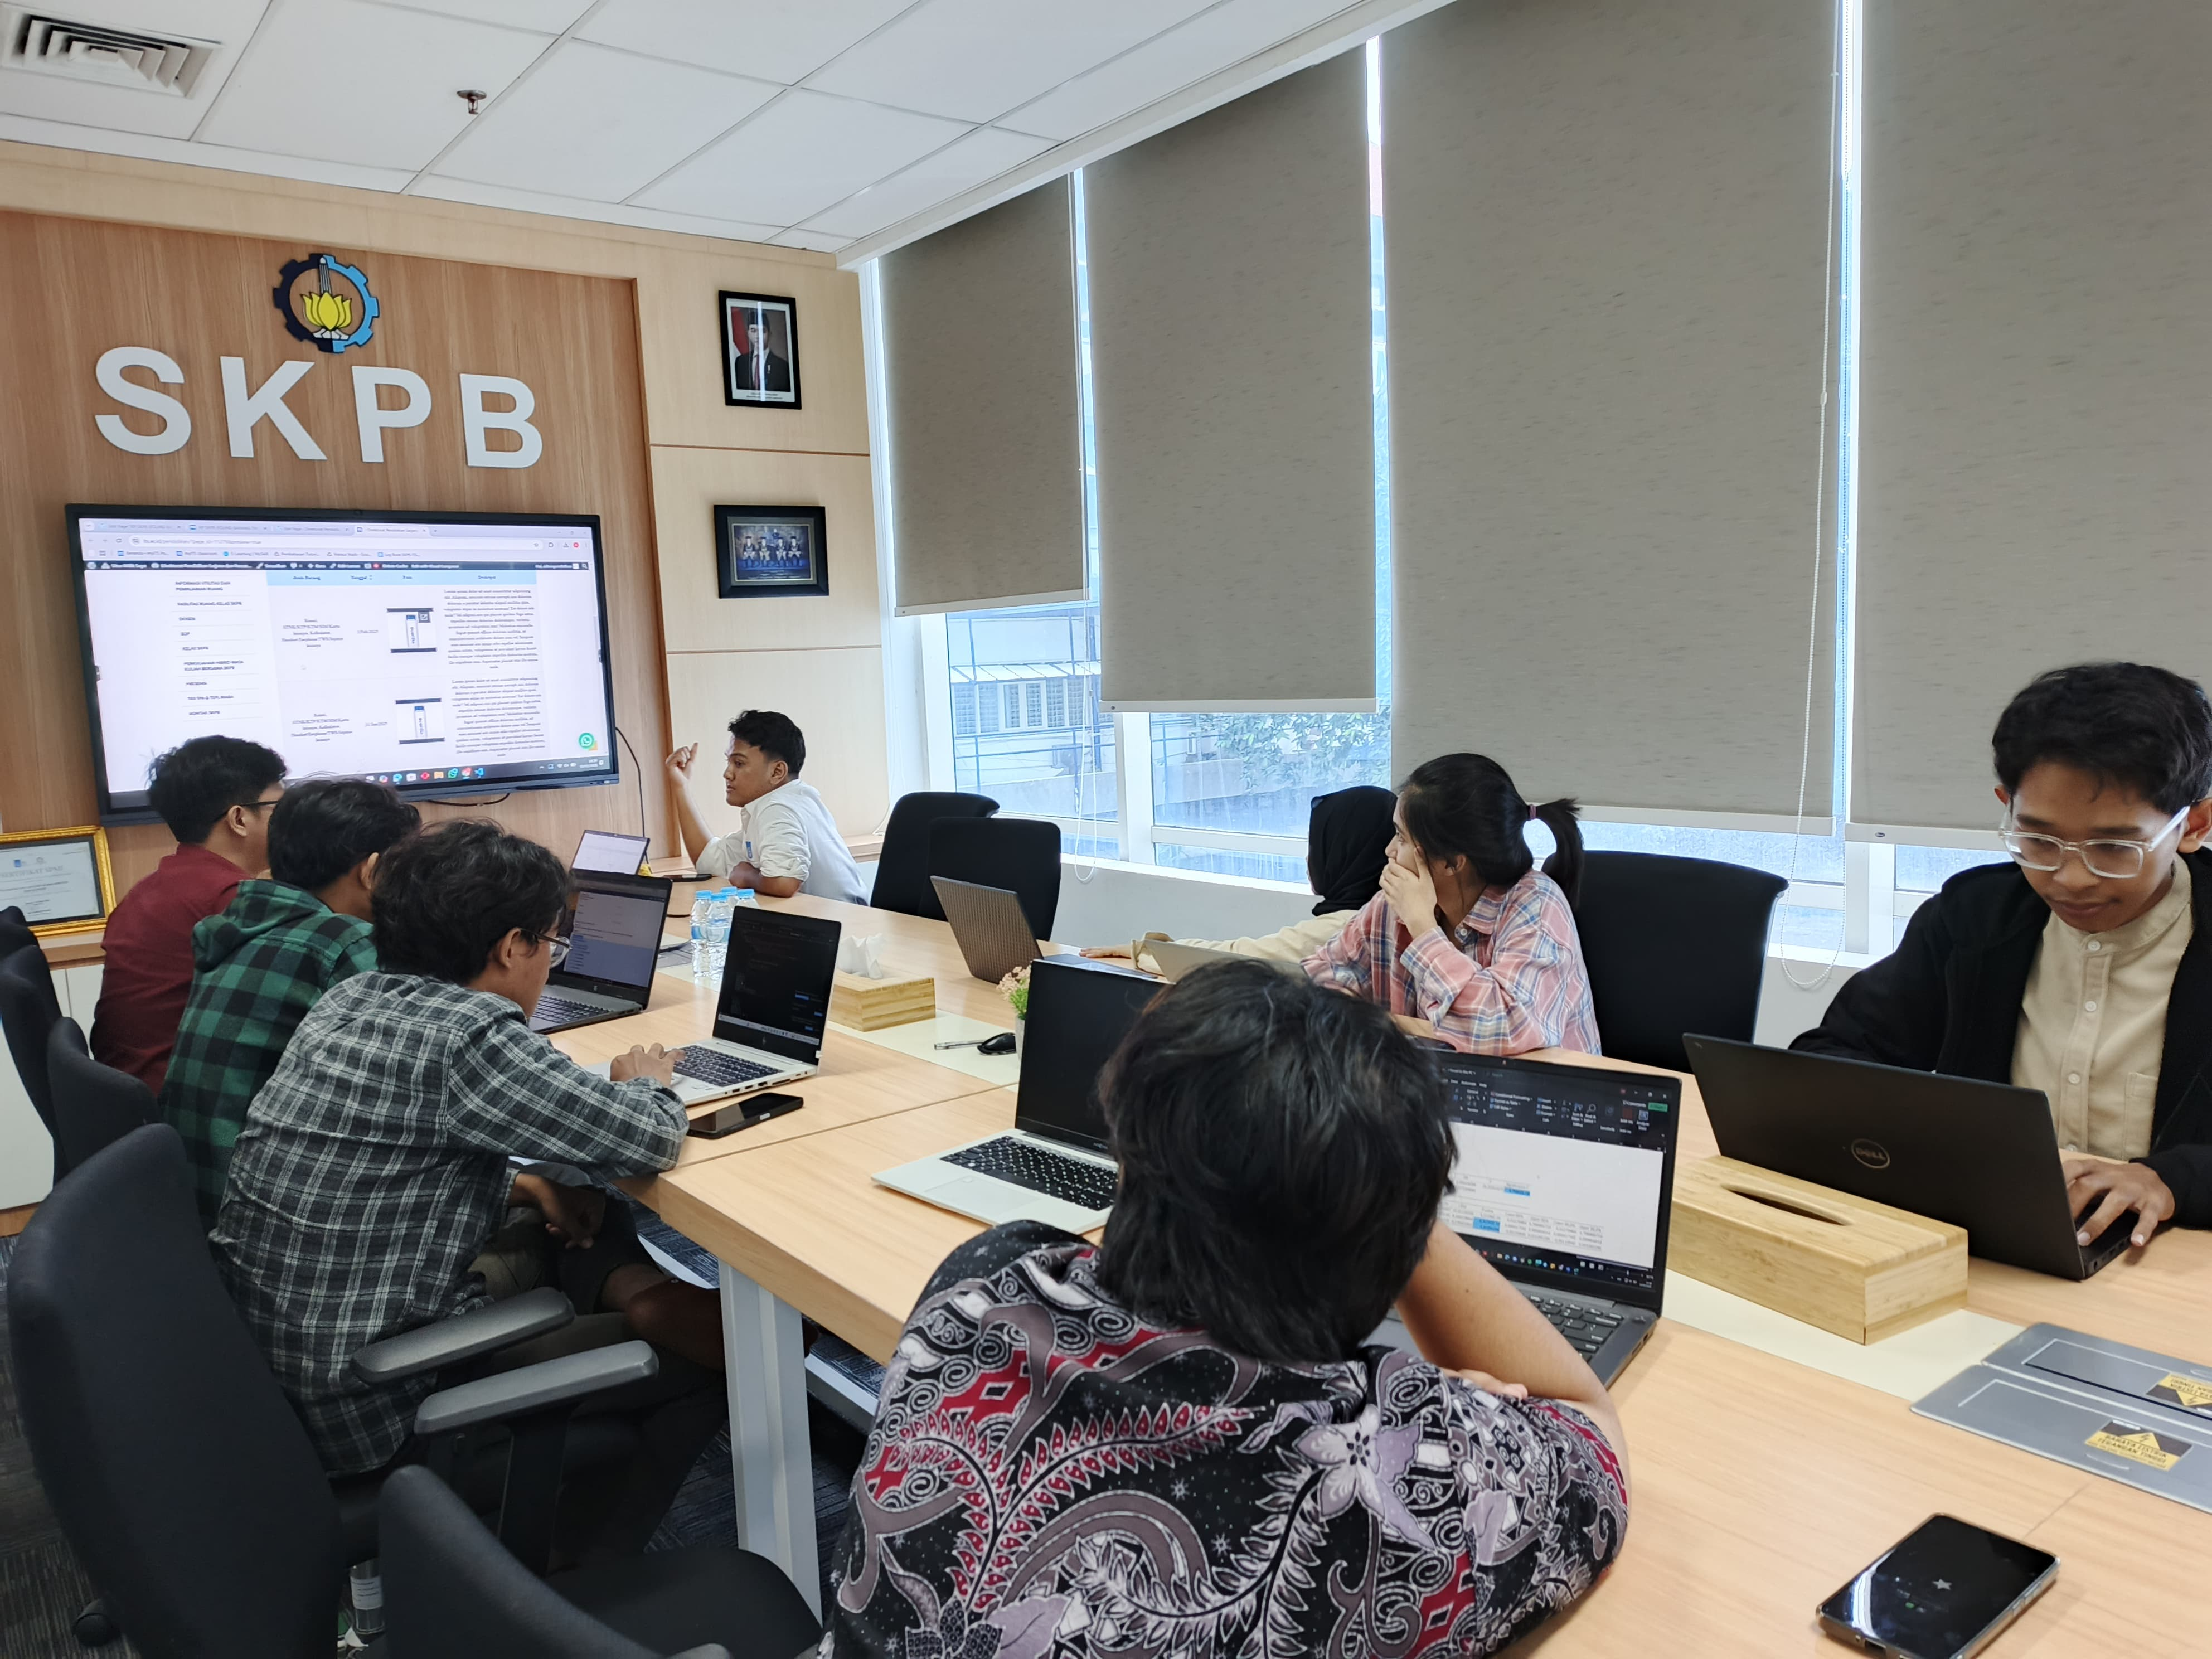
\includegraphics[width=0.8\textwidth]{figs/PemaparanProgres.jpg}
            };
            \end{tikzpicture}

        \column{0.05\textwidth}
    \end{columns}
\end{frame}

\subsection{Struktur Organisasi}

\begin{frame}
    \frametitle{\insertsubsection}
    \begin{figure}[h!]
    \centering
    \begin{tikzpicture}[
    node distance=0.8cm and 0.8cm,
    dosen/.style={rectangle, rounded corners=2pt, minimum width=2cm, minimum height=1.2cm, align=center, text=white, draw=none,shade,
      top color=dosen,
      bottom color=dosen,
      rounded corners=6pt,
      blur shadow={shadow blur steps=5},font=\itshape\bfseries\tiny,text width=3cm},
    tendik/.style={rectangle, rounded corners=2pt, minimum width=2cm, minimum height=1.2cm, align=center, text=white, draw=none,shade,
      top color=tendik,
      bottom color=tendik,
      rounded corners=6pt,
      blur shadow={shadow blur steps=5},font=\itshape\bfseries\tiny,text width=3cm},
    line/.style={draw, thick,line cap=rect}
]

% Root
\node[dosen] (root) {DIREKTUR PENGEMBANGAN AKADEMIK DAN INOVASI PEMBELAJARAN};
\node[draw=none, above=of root, yshift=-0.9cm] (empty) {};

% Level 1
\node[dosen, below left=of root,] (d1) {KEPALA SUBDIT KOORDINASI PERKULIAHAN BERSAMA};
\node[dosen, below=of root] (d2) {KEPALA SUBDIT PENGEMBANGAN AKADEMIK DAN KERJASAMA};
\node[dosen, below right=of root,] (d3) {KEPALA SUBDIT PENGEMBANGAN KURIKULUM DAN INOVASI PEMBELAJARAN};

% Tendik bawah d2
\node[tendik, below=of d2] (t1) {MANAJER KERJASAMA AKADEMIK};

% Tendik bawah d3
\node[dosen, below=of d3,xshift=1.4cm] (d4) {KEPALA SEKSI EVALUASI DAN PENGEMBANGAN METODE PEMBELAJARAN};
\node[dosen, below=of d4,yshift=0.5cm] (d5) {KEPALA SEKSI EVALUASI DAN PENGEMBANGAN TEKNOLOGI PEMBELAJARAN};

% Keterangan posisi
\node[dosen,minimum width=0.5cm,text width=1cm, minimum height=0.4cm, below=of d1, yshift=-1.5cm,xshift=-1cm] (pos1) {$\,$};
\node[tendik,minimum width=0.5cm,text width=1cm, minimum height=0.4cm, below=of d1, yshift=-2cm,xshift=-1cm] (pos2) {$\,$};
\node[above=of pos2, yshift=-0.3cm] (pos3) {\tiny\sffamily Catatan:};
\node[right=of pos1, xshift=-0.75cm] (pos4) {\tiny\sffamily\color{dosen} Jabatan diisi Dosen};
\node[right=of pos2, xshift=-0.75cm] (pos5) {\tiny\sffamily\color{tendik} Jabatan diisi Tendik};

% Draw lines
\draw[line] (root) |-++(0,-1.2) -| (d1);
\draw[line] (root) -- (d2);
\draw[line] (root) |-++(0,-1.2) -| (d3);
\draw[line] (d2) -- (t1);
\draw[line] (d3) |-++(-0.5,-1.2) |- (d4);
\draw[line] (d3) |-++(-0.5,-1.2) |- (d5);
\end{tikzpicture}
\end{figure}
\end{frame}

\section{Pelaksanaan Kerja Praktik}

\setLayout{horizontal}
\subsection{\textit{Project} Kerja Praktik}

\begin{frame}
    \frametitle{\insertsubsection}
    \begin{figure}[h]
        \centering
        \begin{subfigure}[t]{0.5\textwidth}
            \centering
            \begin{tikzpicture}
            \node[draw=black, drop shadow, line width=1pt, inner sep=0] {
              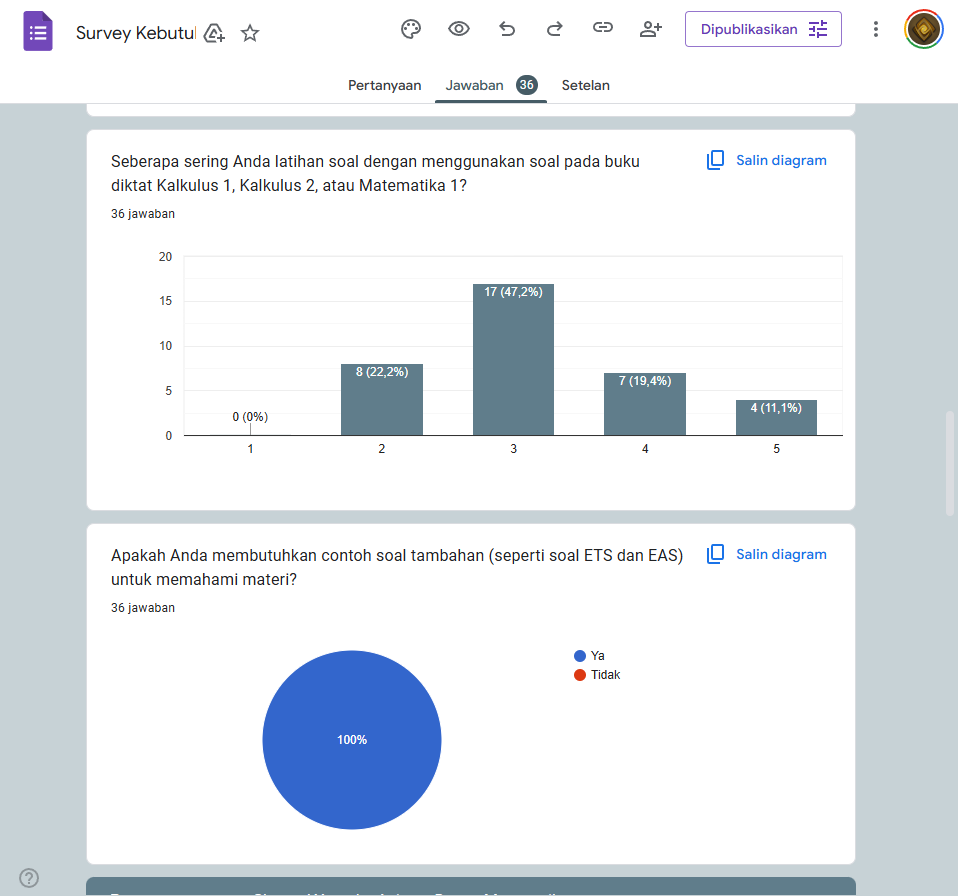
\includegraphics[height=1.7in]{figs/Web4.png}
            };
            \end{tikzpicture}
        \end{subfigure}%
        \begin{subfigure}[t]{0.5\textwidth}
            \centering
            \begin{tikzpicture}
            \node[draw=black, drop shadow, line width=1pt, inner sep=0] {
              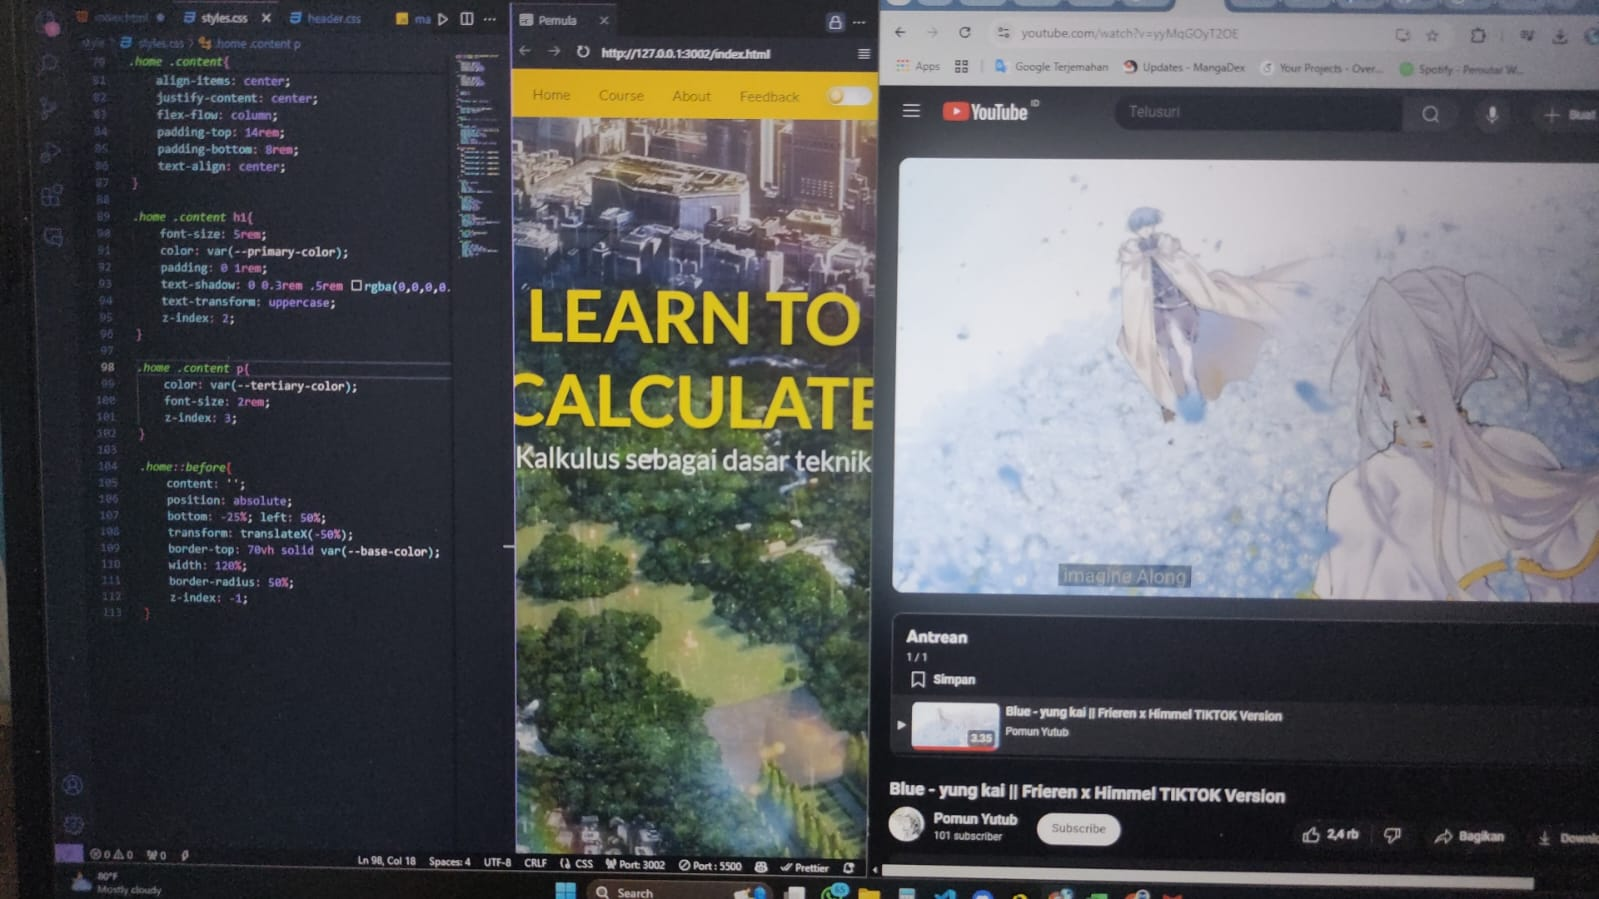
\includegraphics[height=1.7in]{figs/Web1.jpg}
            };
            \end{tikzpicture}
        \end{subfigure}
        \caption{Hasil survey dan trial belajar membuat website} 
    \end{figure}
\end{frame}


\begin{frame}
    \begin{figure}[h]
    \centering
    \begin{subfigure}[t]{0.5\textwidth}
        \centering
        \begin{tikzpicture}
            \node[draw=black, drop shadow, line width=1pt, inner sep=0] {
              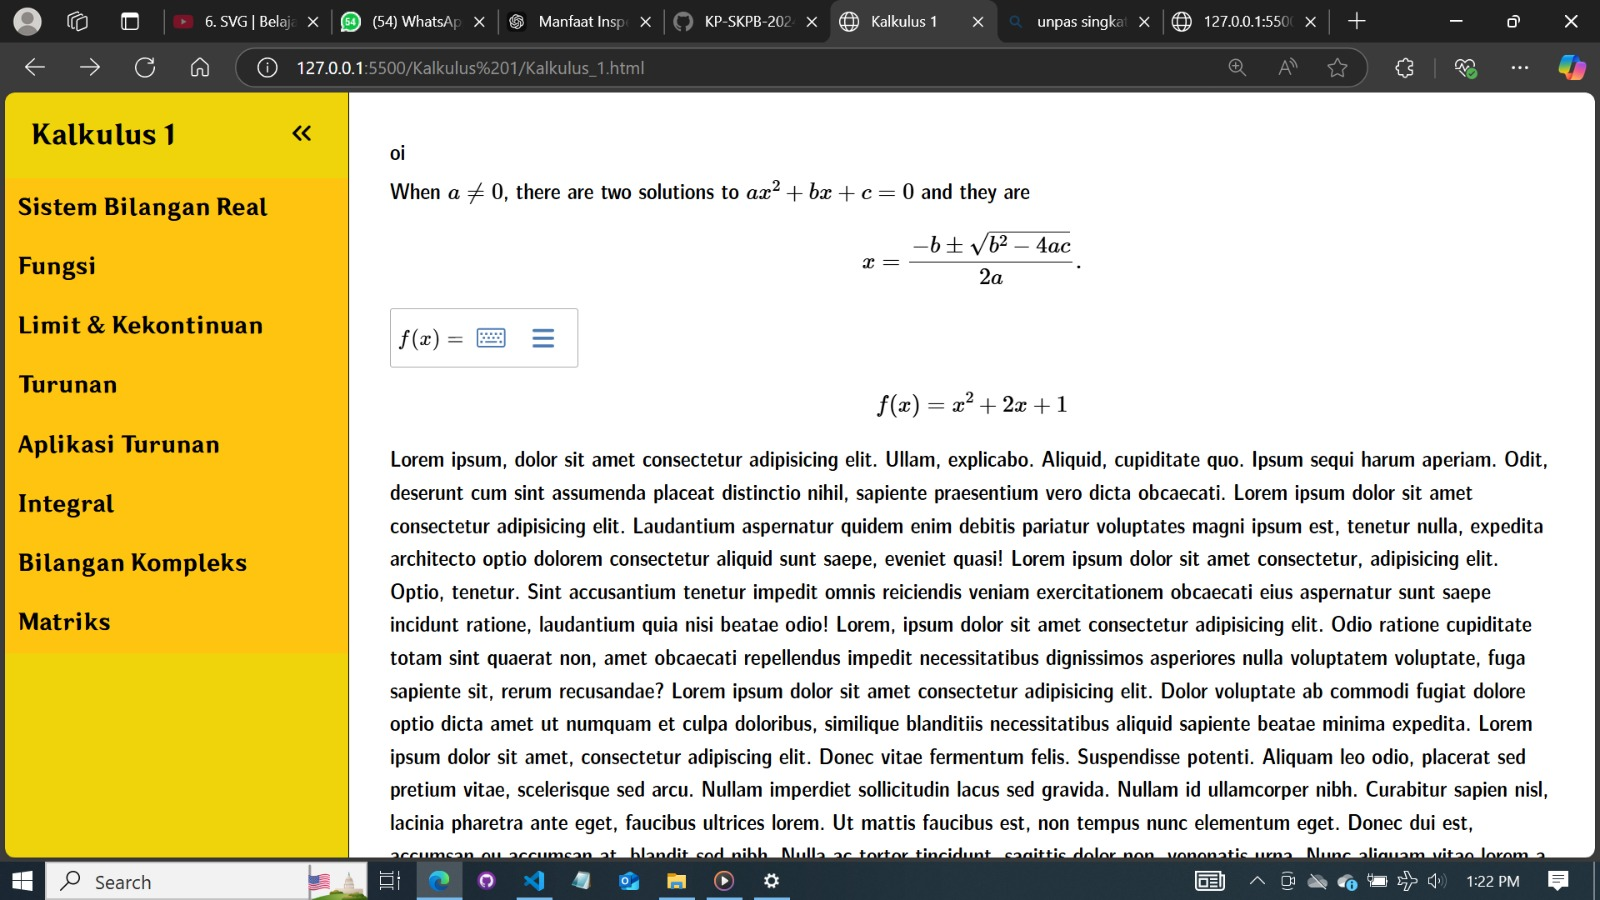
\includegraphics[height=1.7in]{figs/Web2.jpg}
            };
        \end{tikzpicture}
    \end{subfigure}%
    ~ \qquad
    \begin{subfigure}[t]{0.5\textwidth}
        \centering
        \begin{tikzpicture}
            \node[draw=black, drop shadow, line width=1pt, inner sep=0] {
              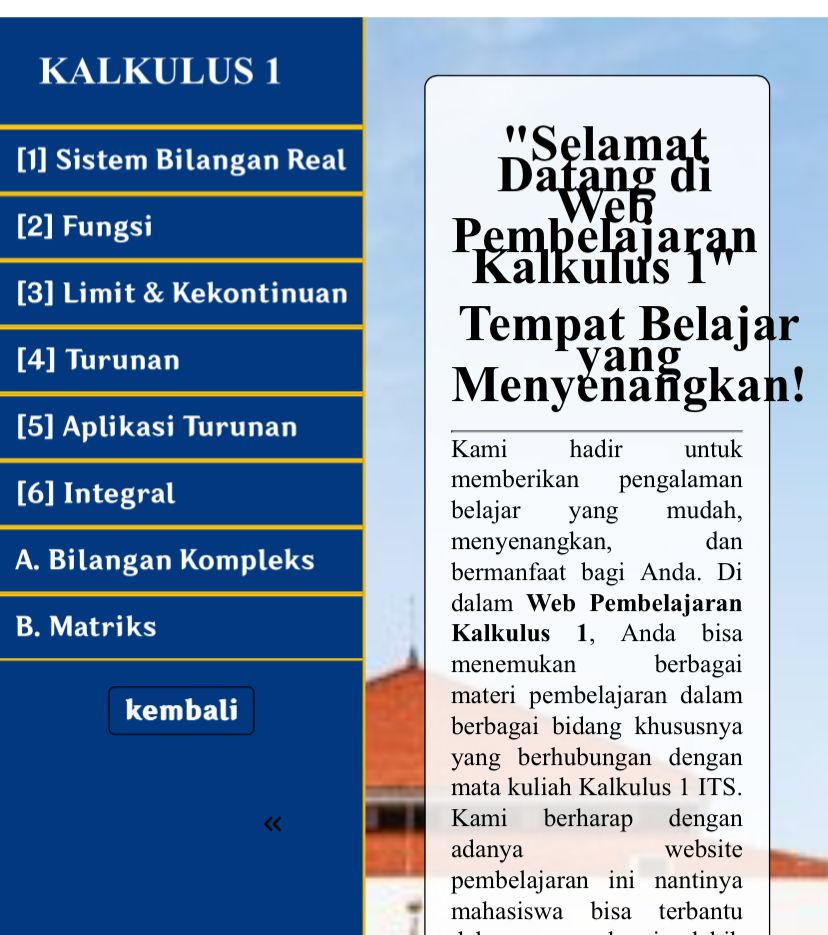
\includegraphics[height=2in]{figs/Web3.jpg}
            };
        \end{tikzpicture}
    \end{subfigure}
    \caption{Tampilan non-finish website kalkulus} 
    \end{figure}
\end{frame}

\begin{frame}
    \begin{figure}[h]
        \centering
        \begin{subfigure}[t]{0.3\textwidth}
            \centering
            \begin{tikzpicture}
                \node[draw=black, drop shadow, line width=1pt, inner sep=0] {
                  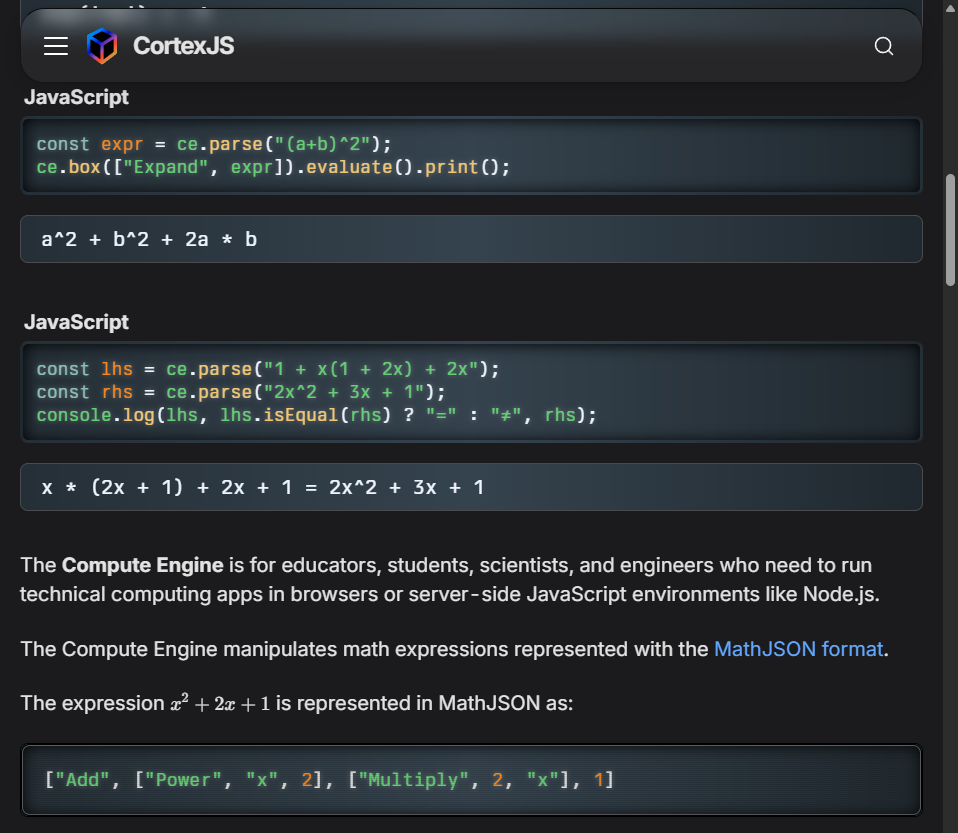
\includegraphics[height=1.2in]{figs/Web5.png}
                };
            \end{tikzpicture}
        \end{subfigure}%
        ~
        \begin{subfigure}[t]{0.3\textwidth}
            \centering
            \begin{tikzpicture}
                \node[draw=black, drop shadow, line width=1pt, inner sep=0] {
                  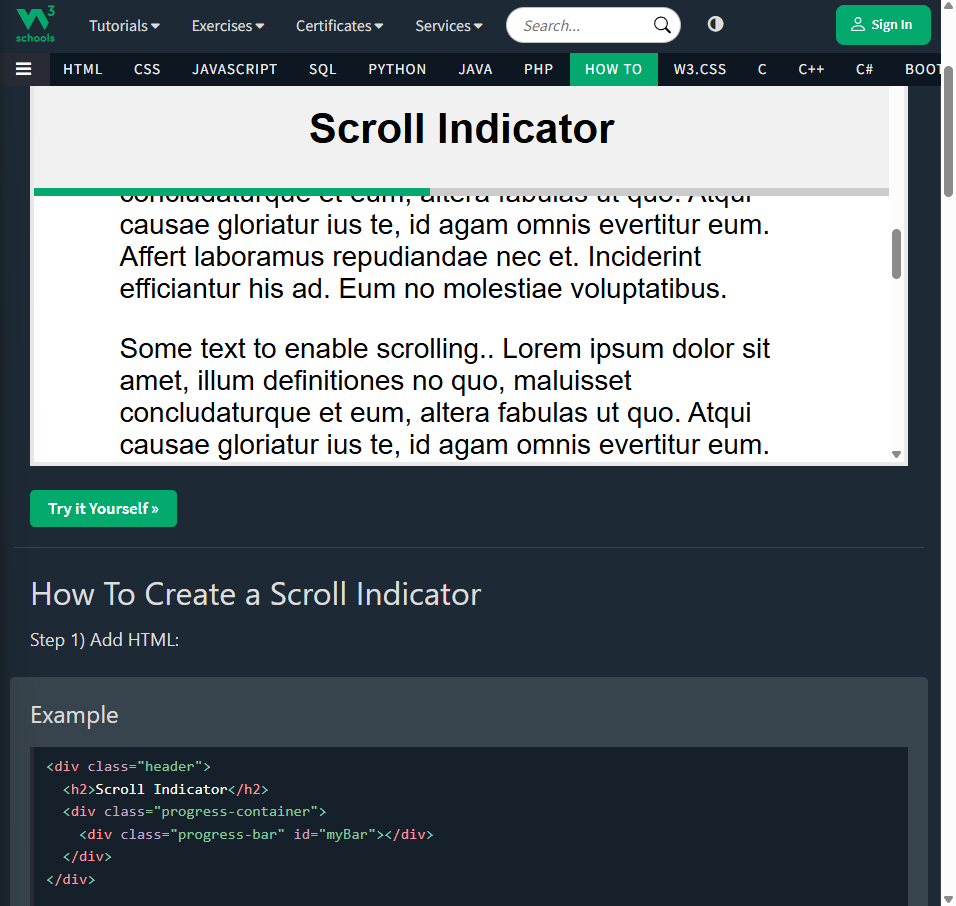
\includegraphics[height=1.2in]{figs/Web6.png}
                };
            \end{tikzpicture}
        \end{subfigure}
        
        \begin{subfigure}[t]{0.3\textwidth}
            \centering
            \begin{tikzpicture}
                \node[draw=black, drop shadow, line width=1pt, inner sep=0] {
                  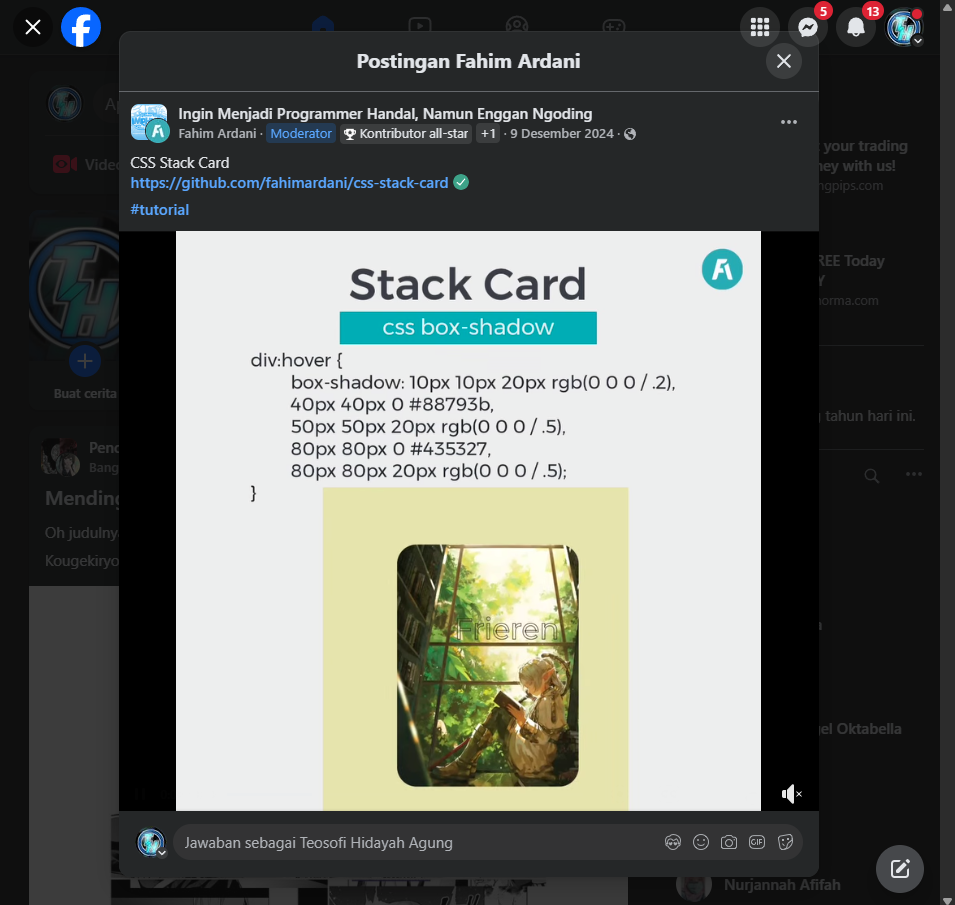
\includegraphics[height=1.3in]{figs/Web7.png}
                };
            \end{tikzpicture}
        \end{subfigure}
        ~
        \begin{subfigure}[t]{0.3\textwidth}
            \centering
            \begin{tikzpicture}
                \node[draw=black, drop shadow, line width=1pt, inner sep=0] {
                  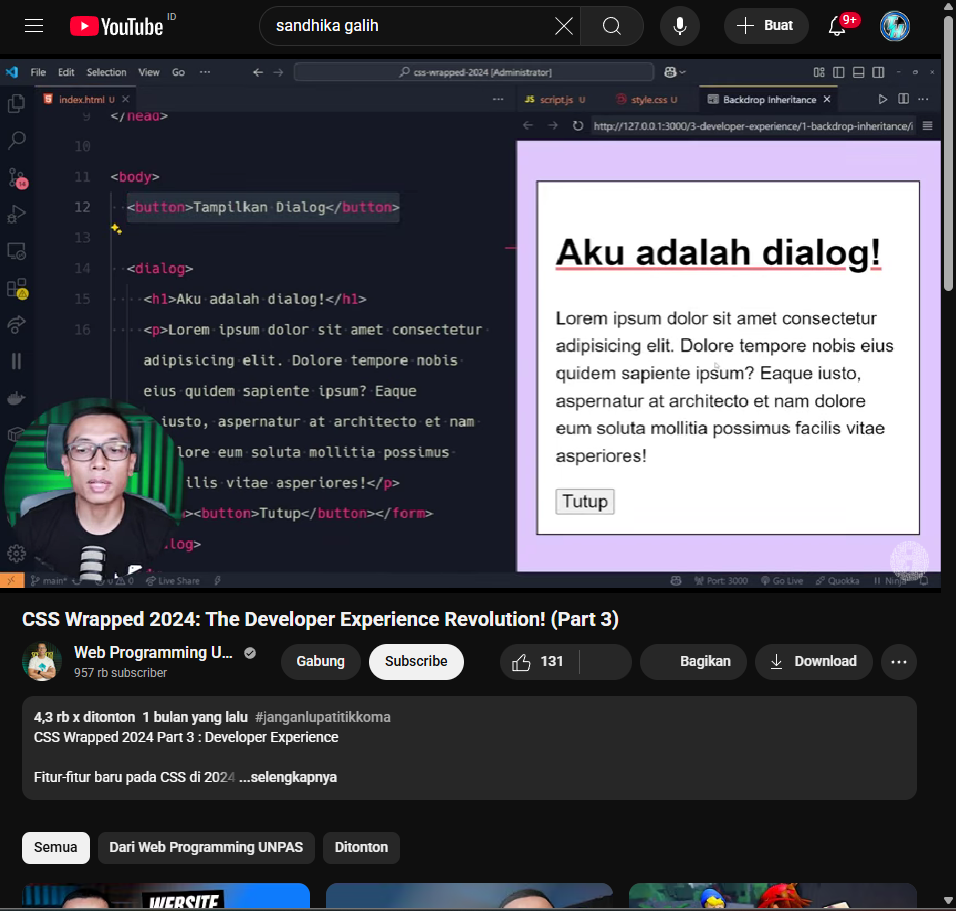
\includegraphics[height=1.3in]{figs/Web8.png}
                };
            \end{tikzpicture}
        \end{subfigure}
        \caption{Mempelajari dokumentasi dan informasi \textit{open source} yang ada}
    \end{figure}
\end{frame}

\subsection{Kegiatan lain selama Kerja Praktik}

\begin{frame}
    \frametitle{\insertsubsection}
    \begin{figure}[h]
    \centering
    \begin{subfigure}[t]{0.3\textwidth}
        \centering
        \begin{tikzpicture}
            \node[draw=black, drop shadow, line width=1pt, inner sep=0] {
              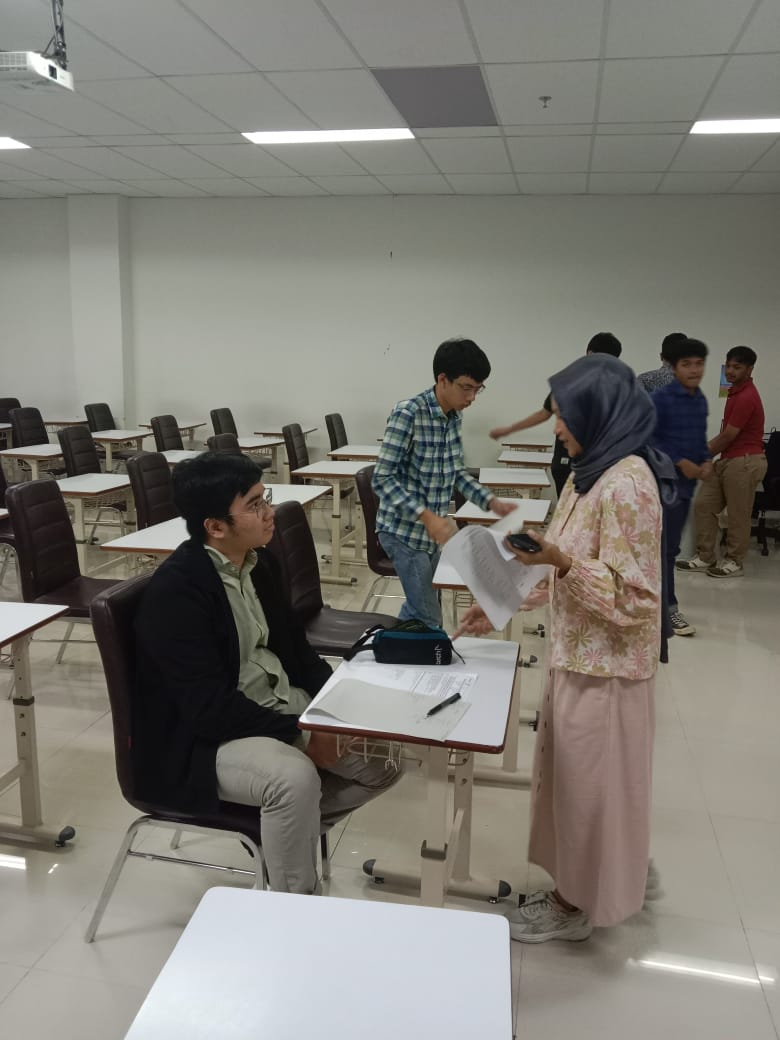
\includegraphics[height=1.7in]{figs/Jaga1.jpg}
            };
        \end{tikzpicture}
    \end{subfigure}%
    ~
    \begin{subfigure}[t]{0.3\textwidth}
        \centering
        \begin{tikzpicture}
            \node[draw=black, drop shadow, line width=1pt, inner sep=0] {
              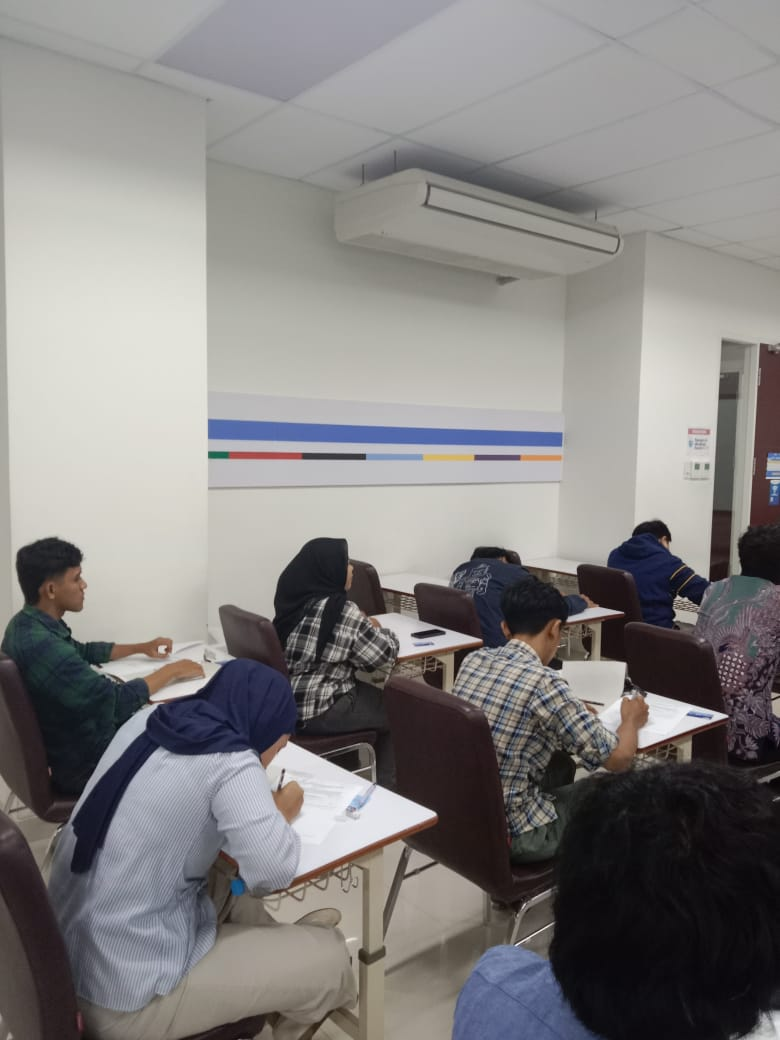
\includegraphics[height=1.7in]{figs/Jaga2.jpg}
            };
        \end{tikzpicture}
    \end{subfigure}
    ~
    \begin{subfigure}[t]{0.3\textwidth}
        \centering
        \begin{tikzpicture}
            \node[draw=black, drop shadow, line width=1pt, inner sep=0] {
              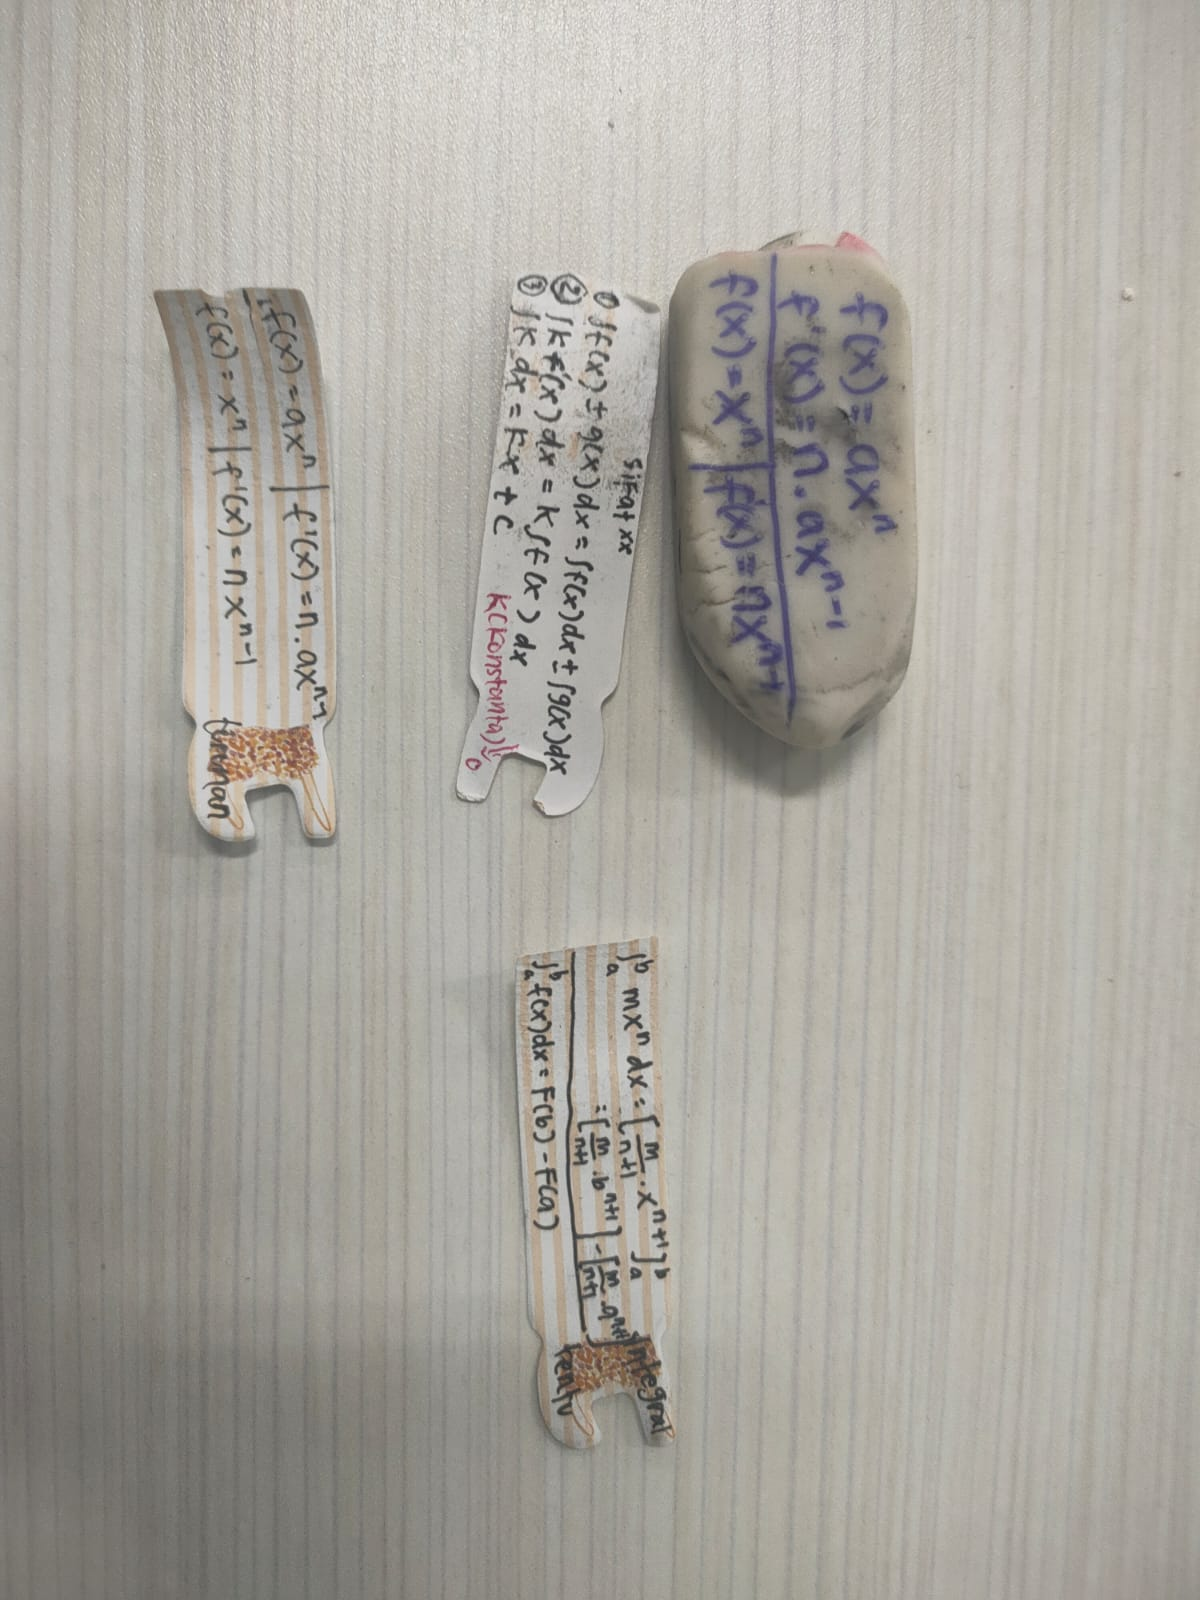
\includegraphics[height=1.7in]{figs/Jaga3.jpg}
            };
        \end{tikzpicture}
    \end{subfigure}
    \caption{Menjaga remidial mahasiswa ulang} 
    \end{figure}
\end{frame}

\begin{frame}
    \vfill
    \begin{figure}[h]
    \centering
    \begin{tikzpicture}
        \node[draw=black, drop shadow, line width=1pt, inner sep=0] {
          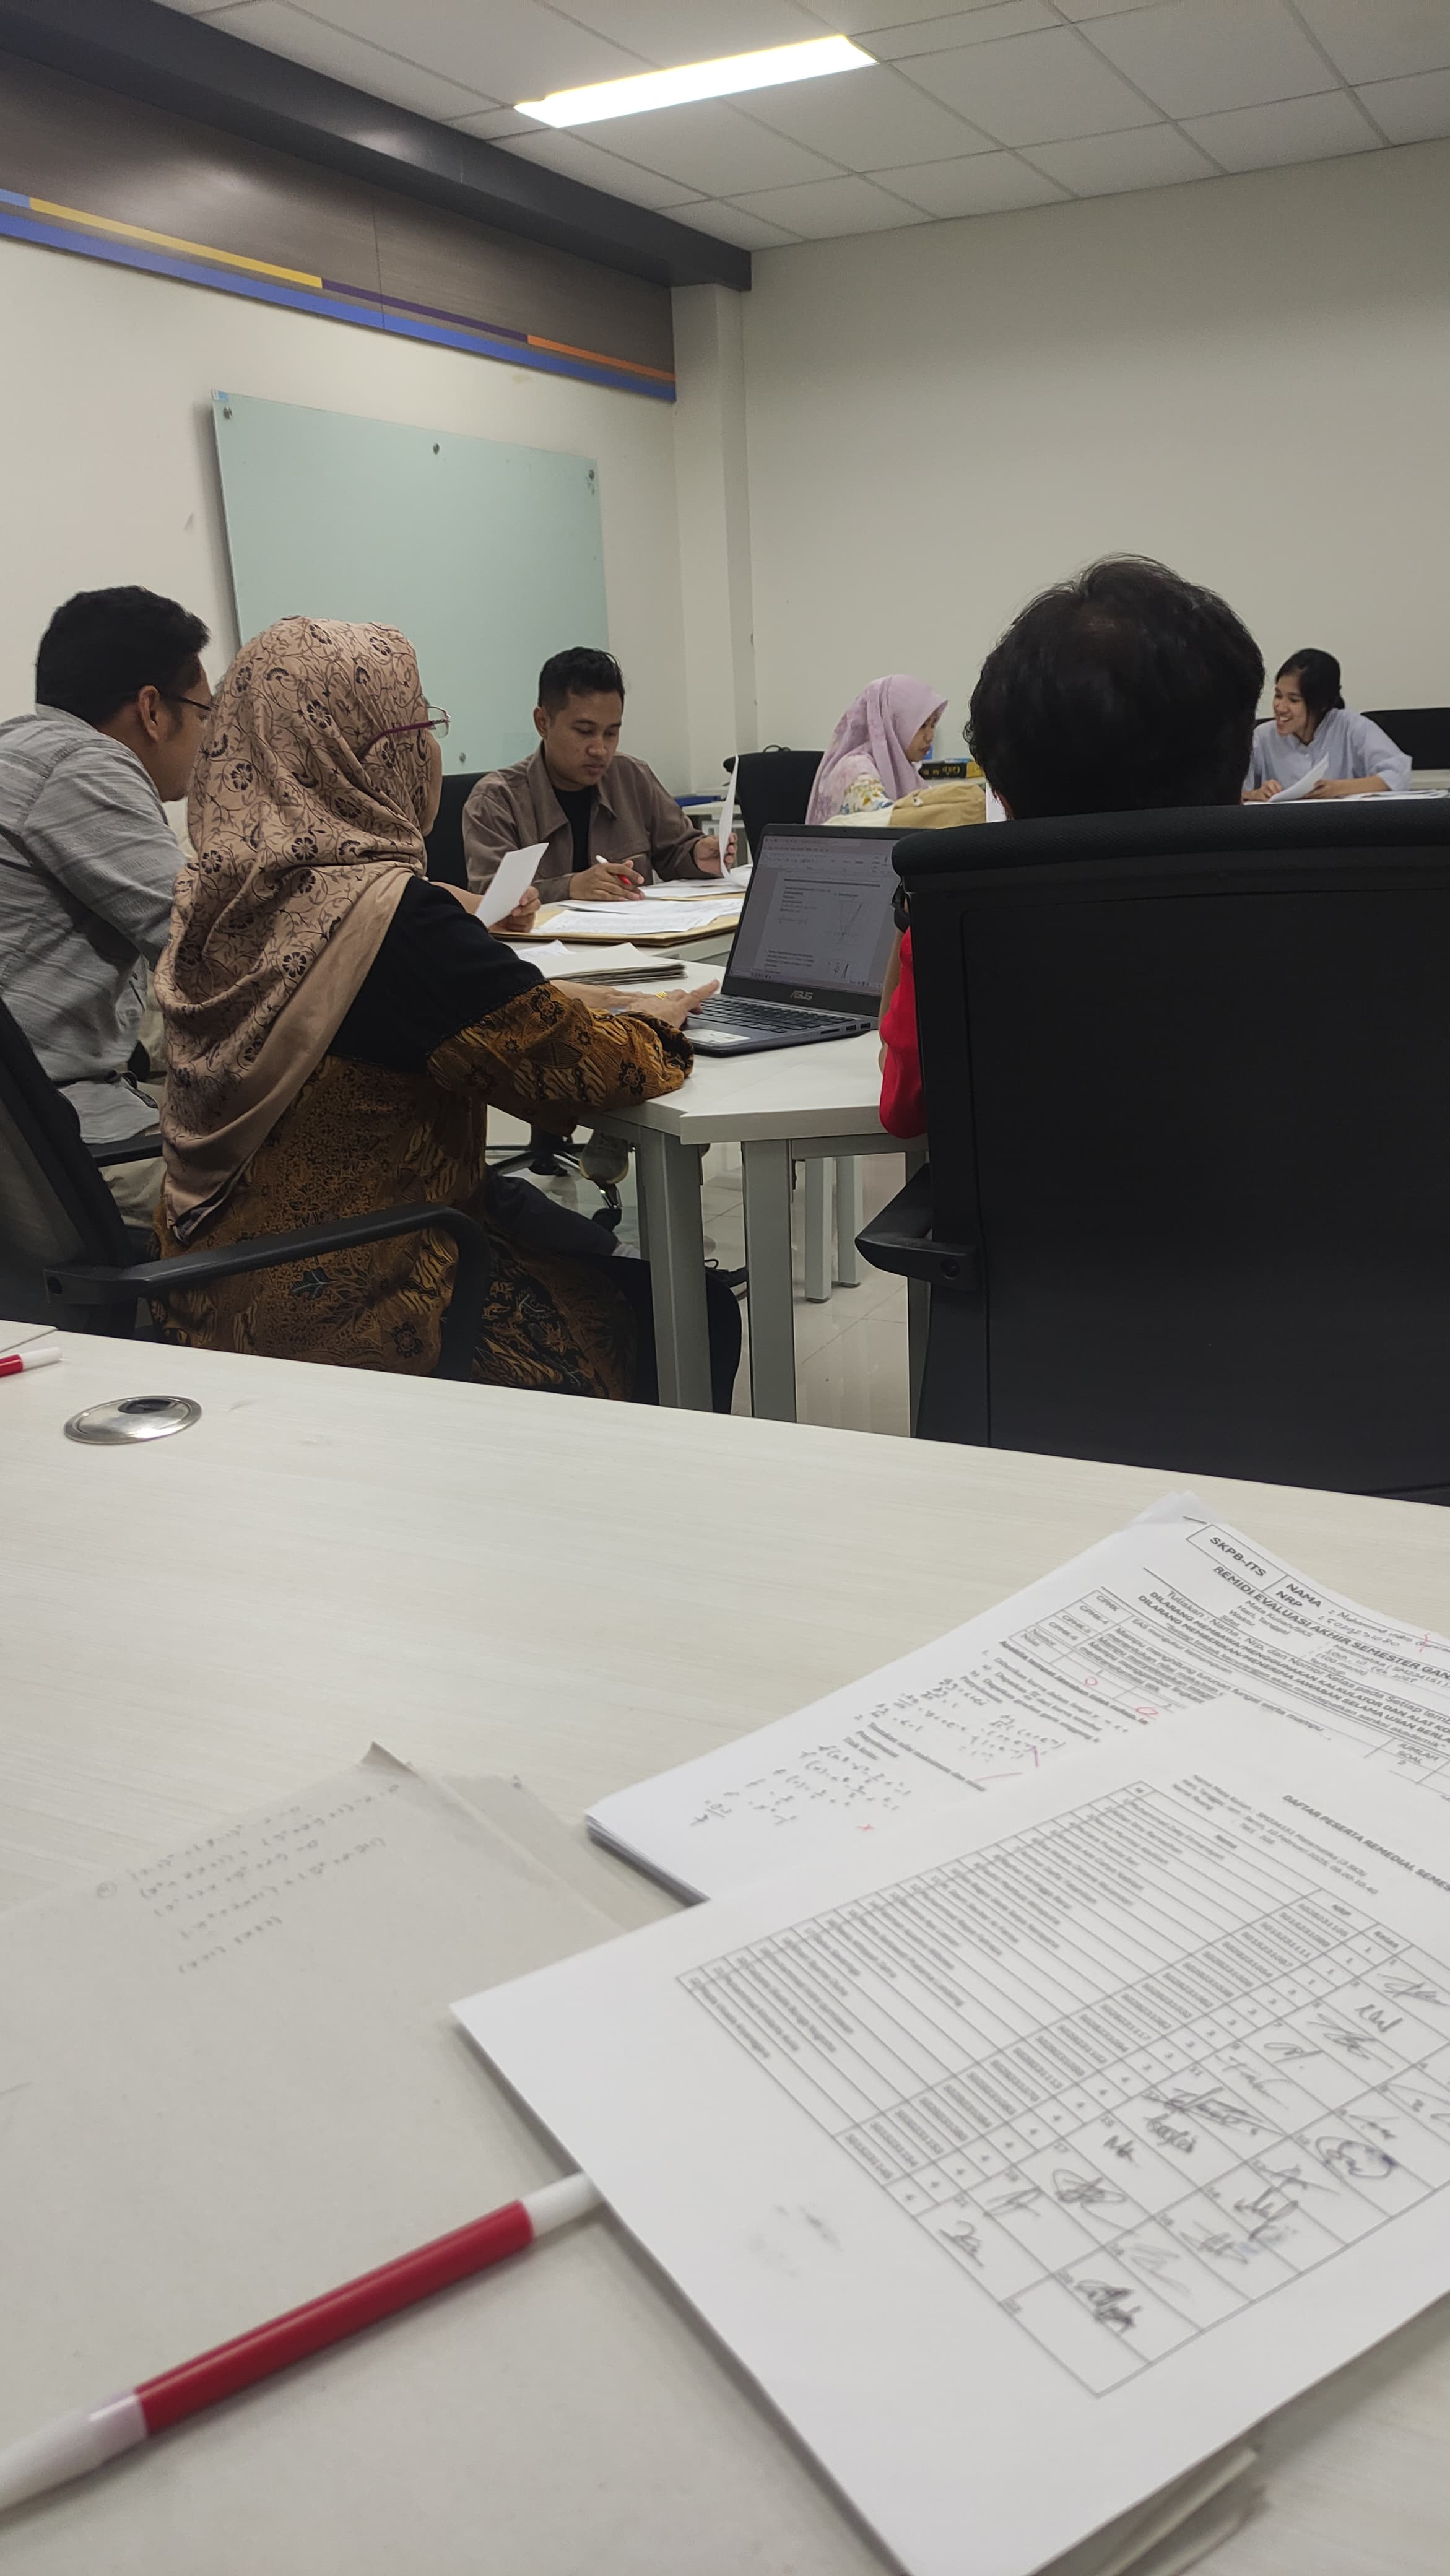
\includegraphics[height=1.6in]{figs/Koreksi1.jpg}
        };
    \end{tikzpicture}
    \begin{tikzpicture}
        \node[draw=black, drop shadow, line width=1pt, inner sep=0] {
          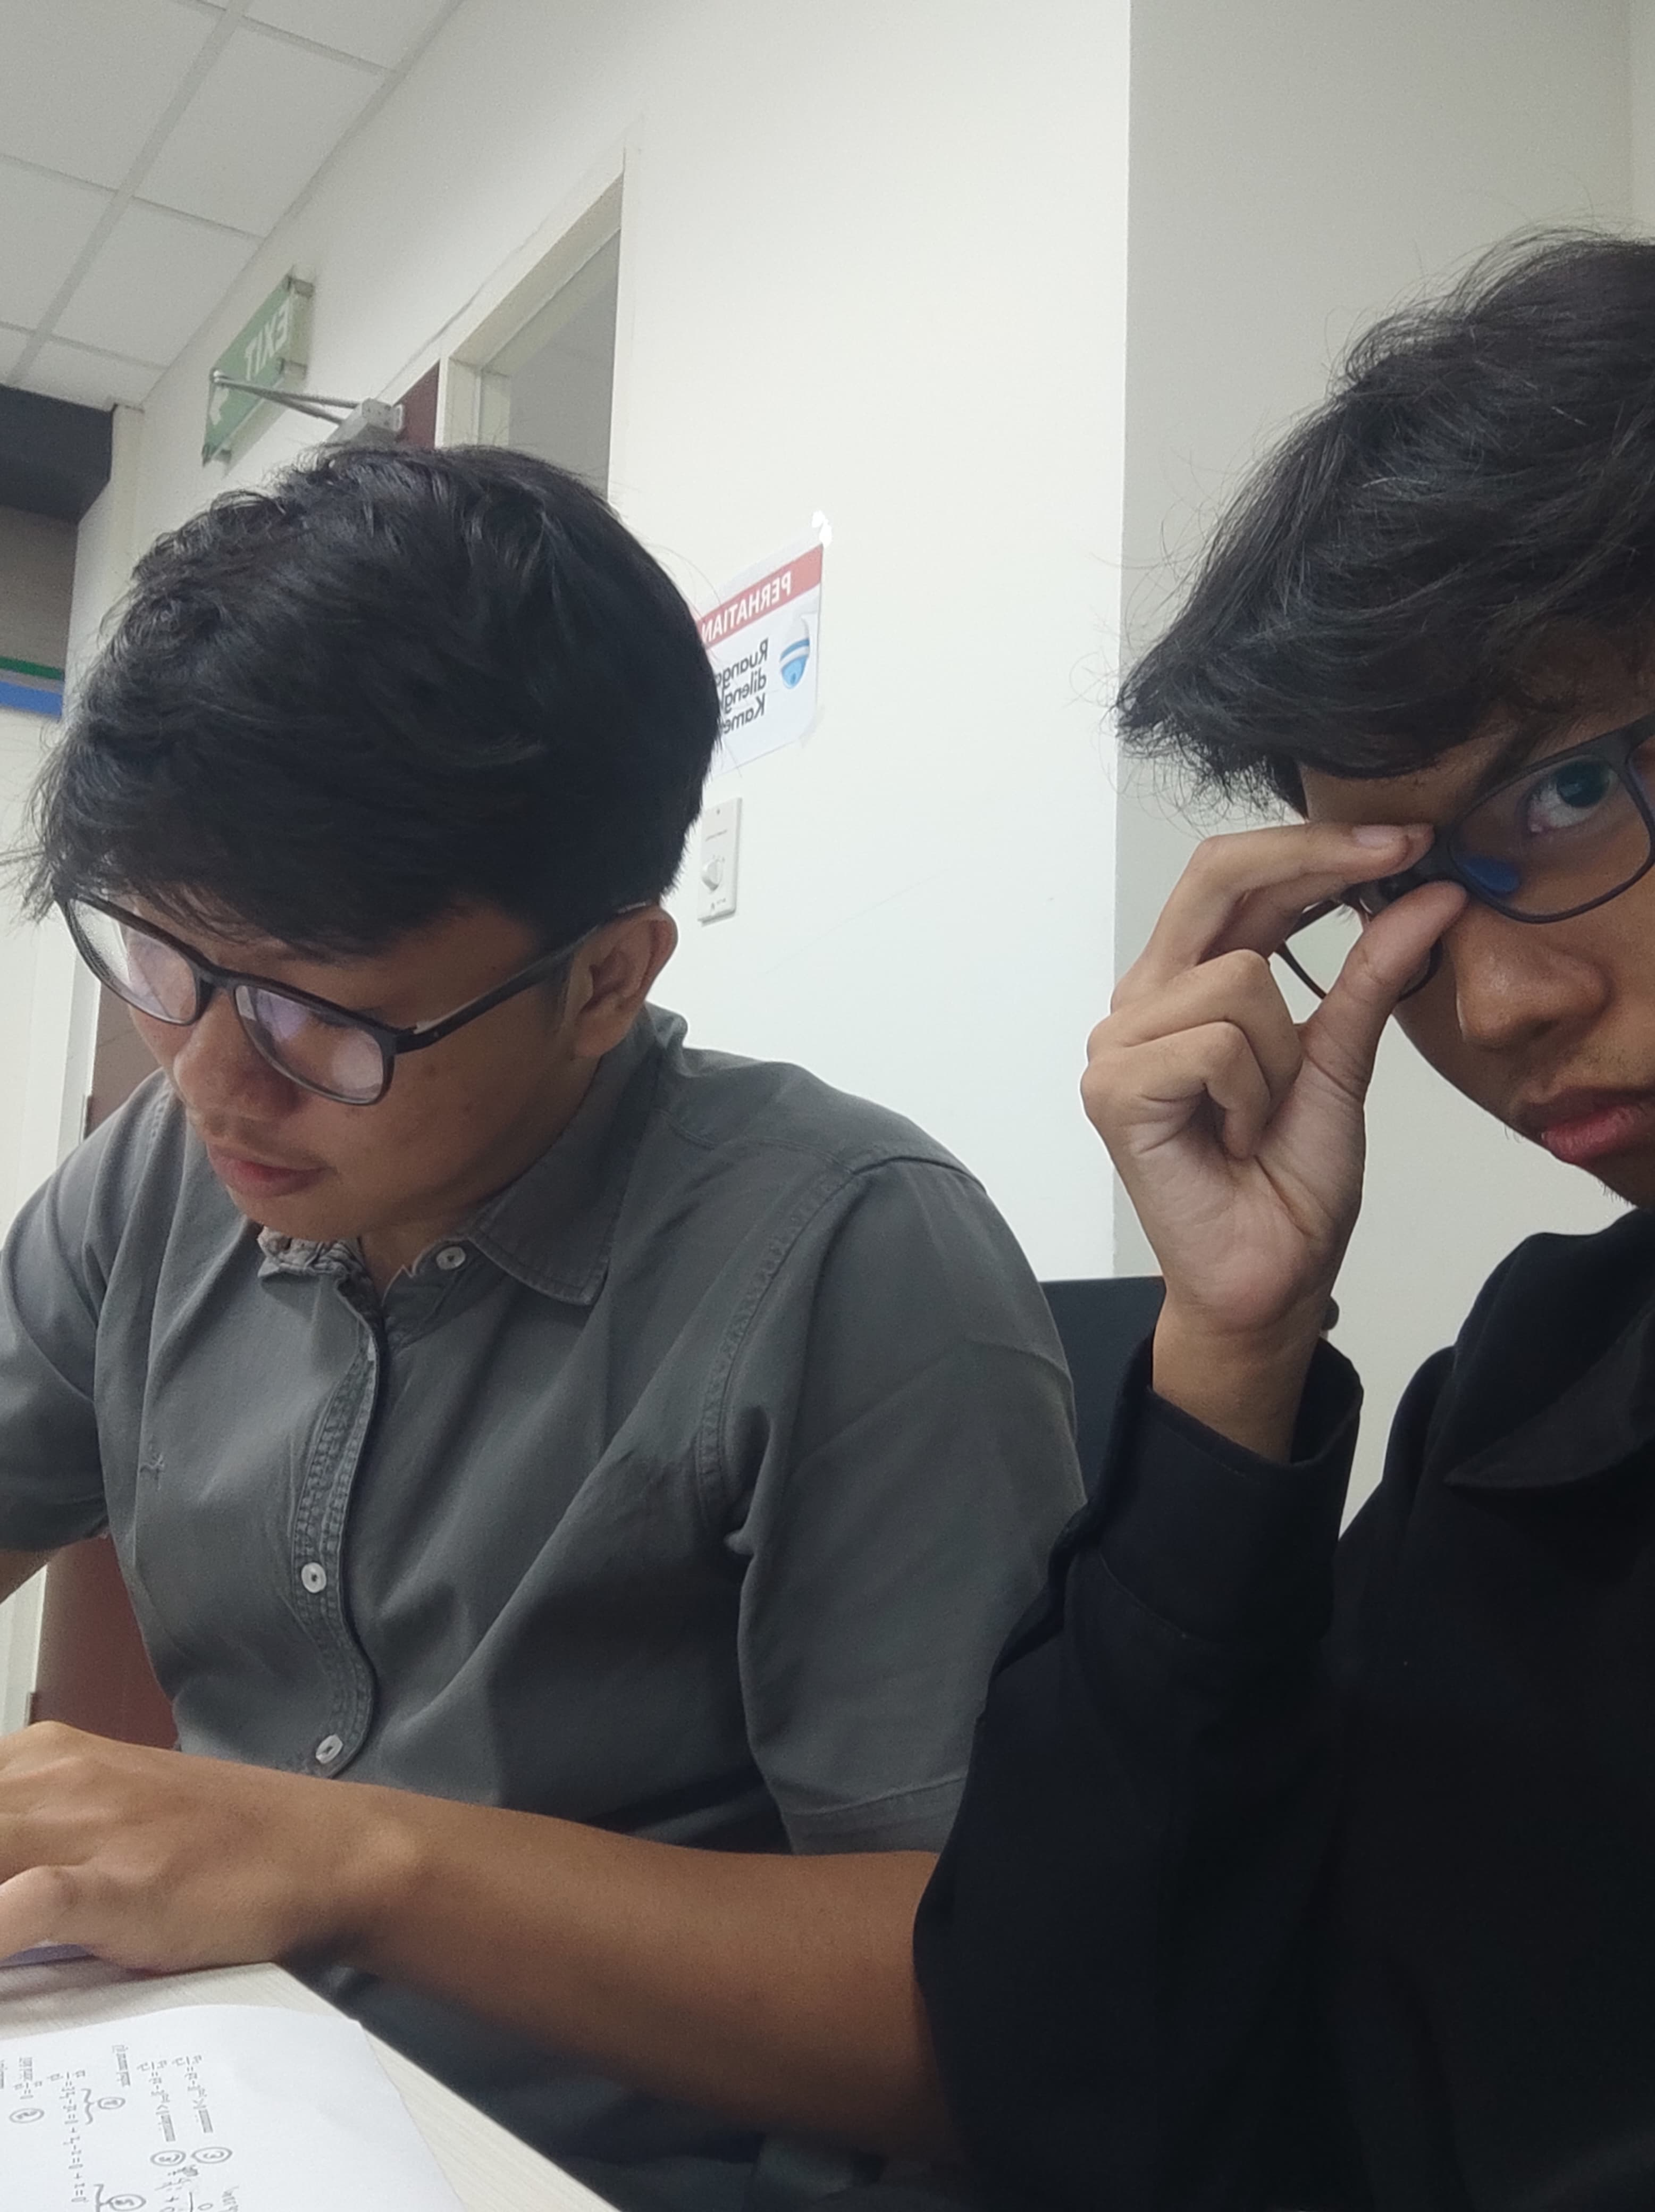
\includegraphics[height=1.6in]{figs/Koreksi2.jpg}
        };
    \end{tikzpicture}
    \begin{tikzpicture}
        \node[draw=black, drop shadow, line width=1pt, inner sep=0] {
          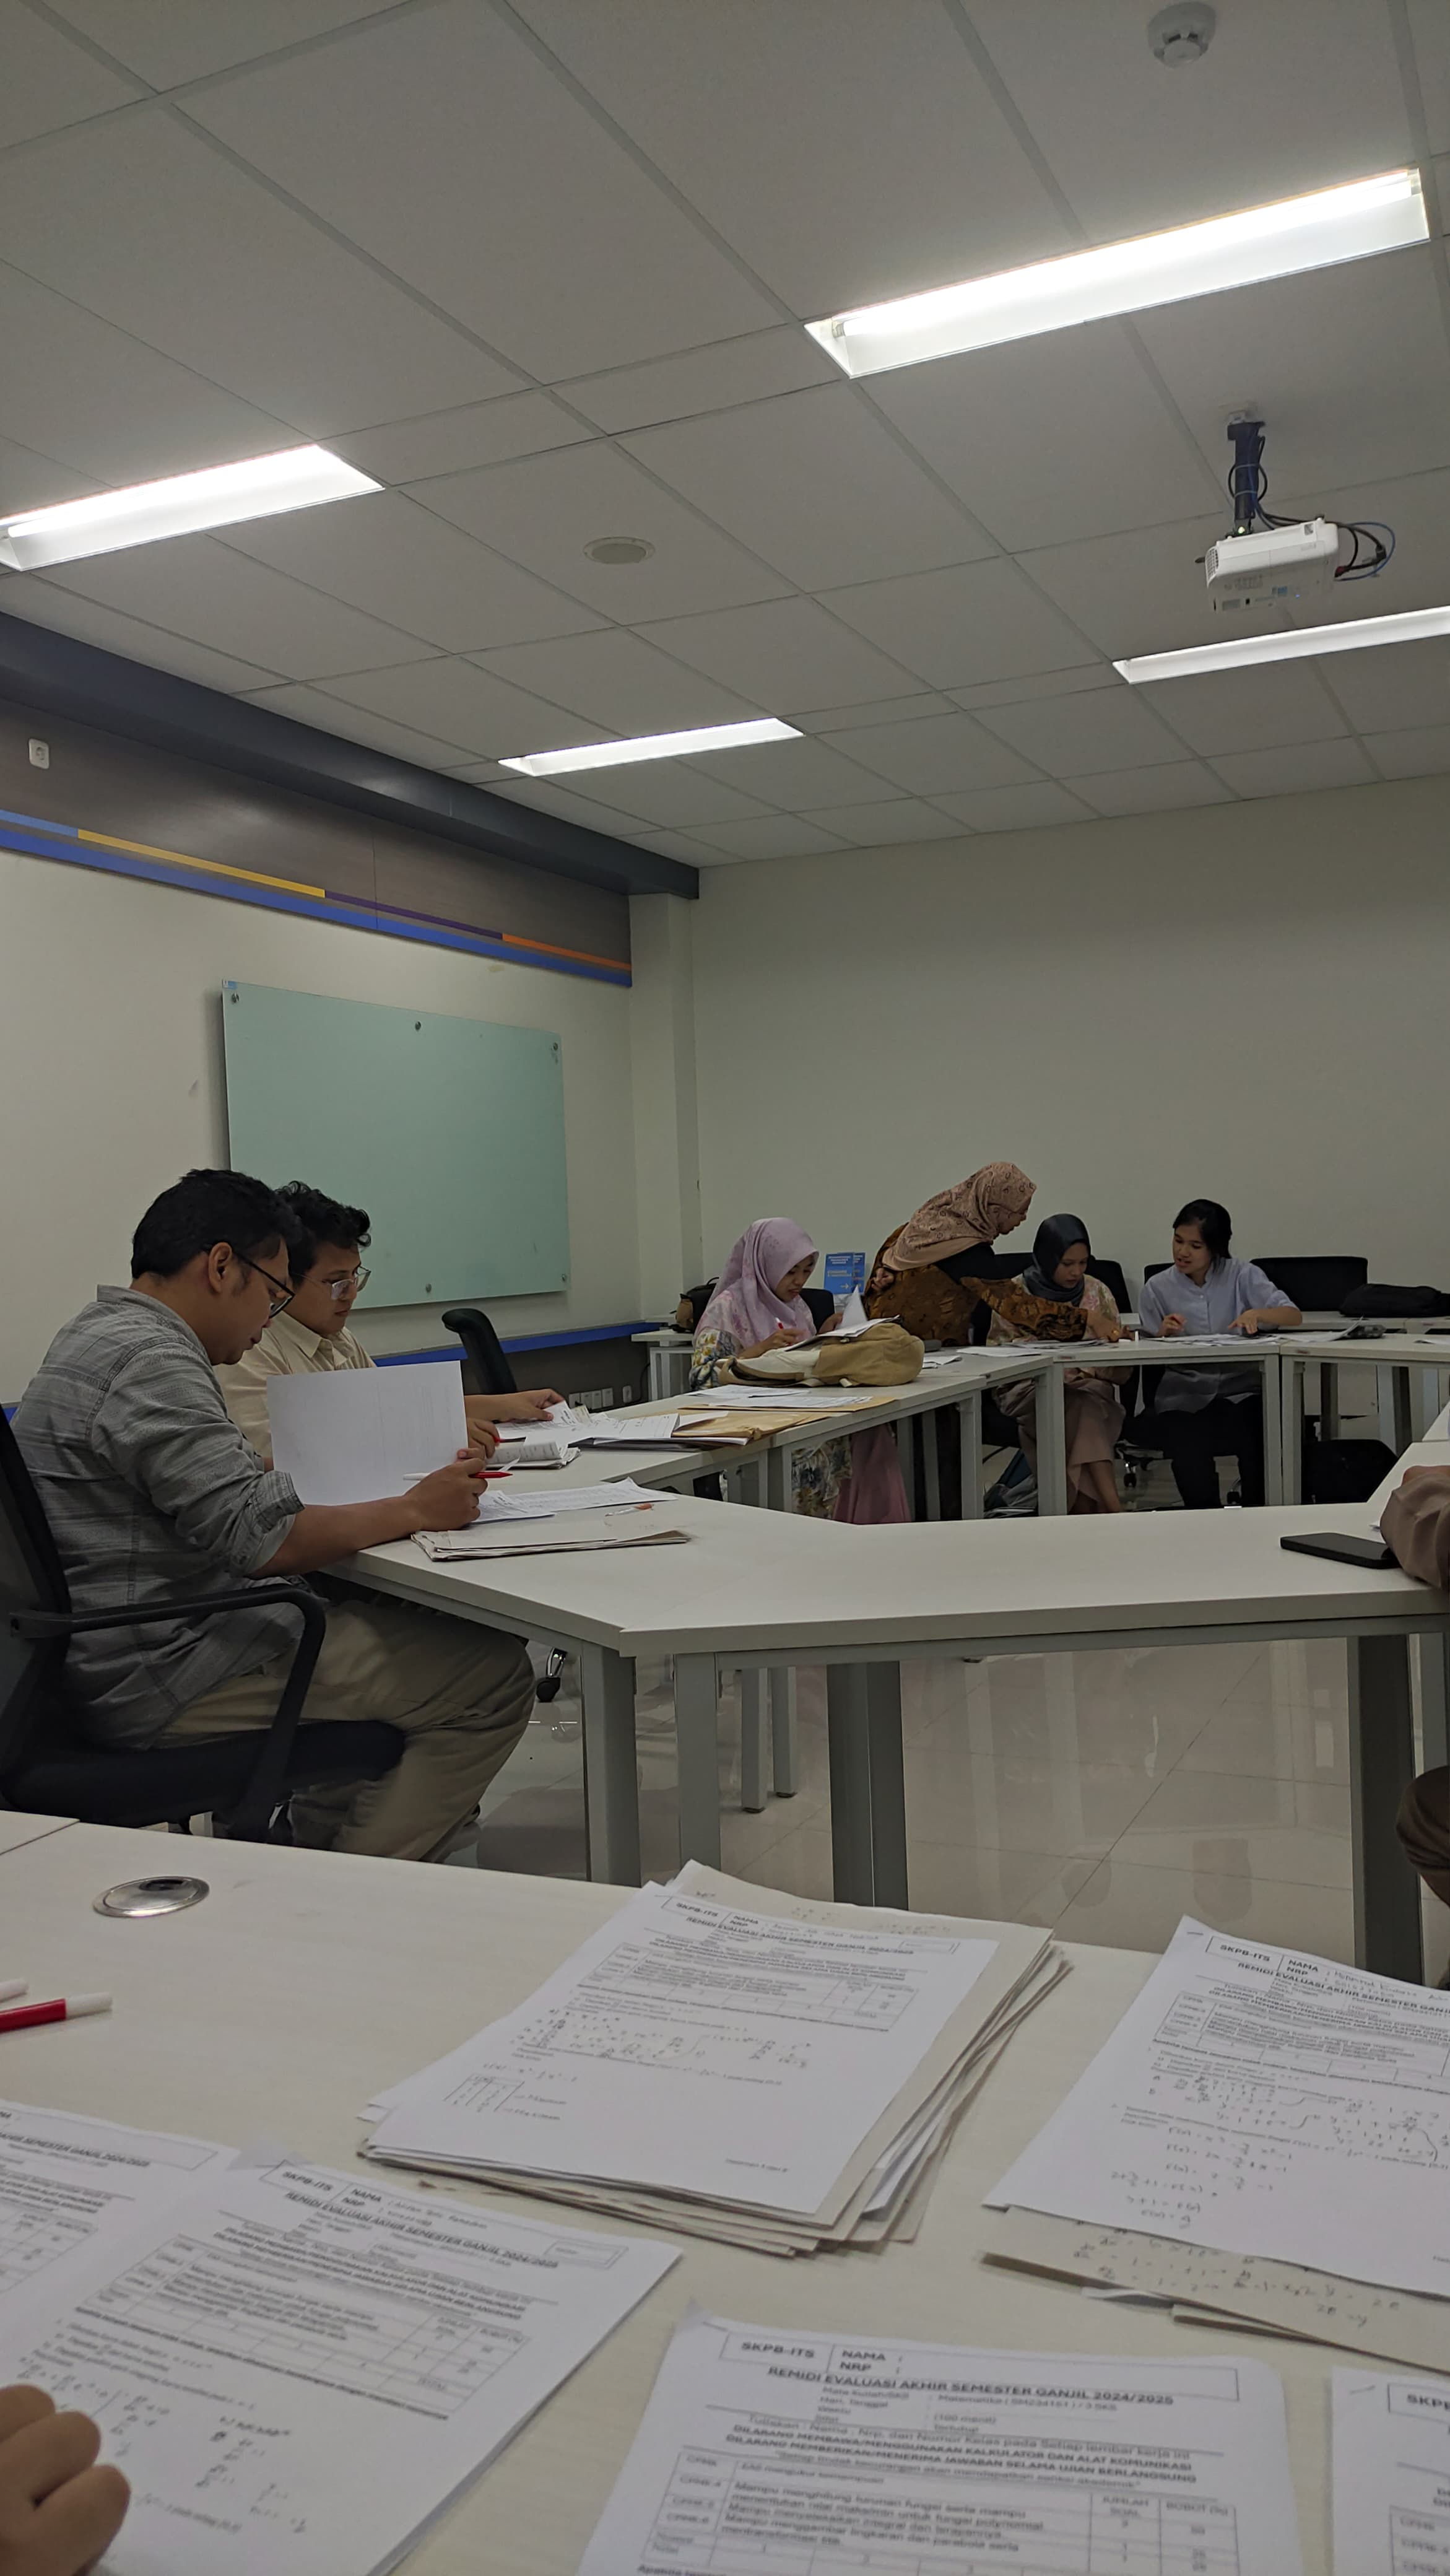
\includegraphics[height=1.6in]{figs/Koreksi3.jpg}
        };
    \end{tikzpicture}
    \begin{tikzpicture}
        \node[draw=black, drop shadow, line width=1pt, inner sep=0] {
          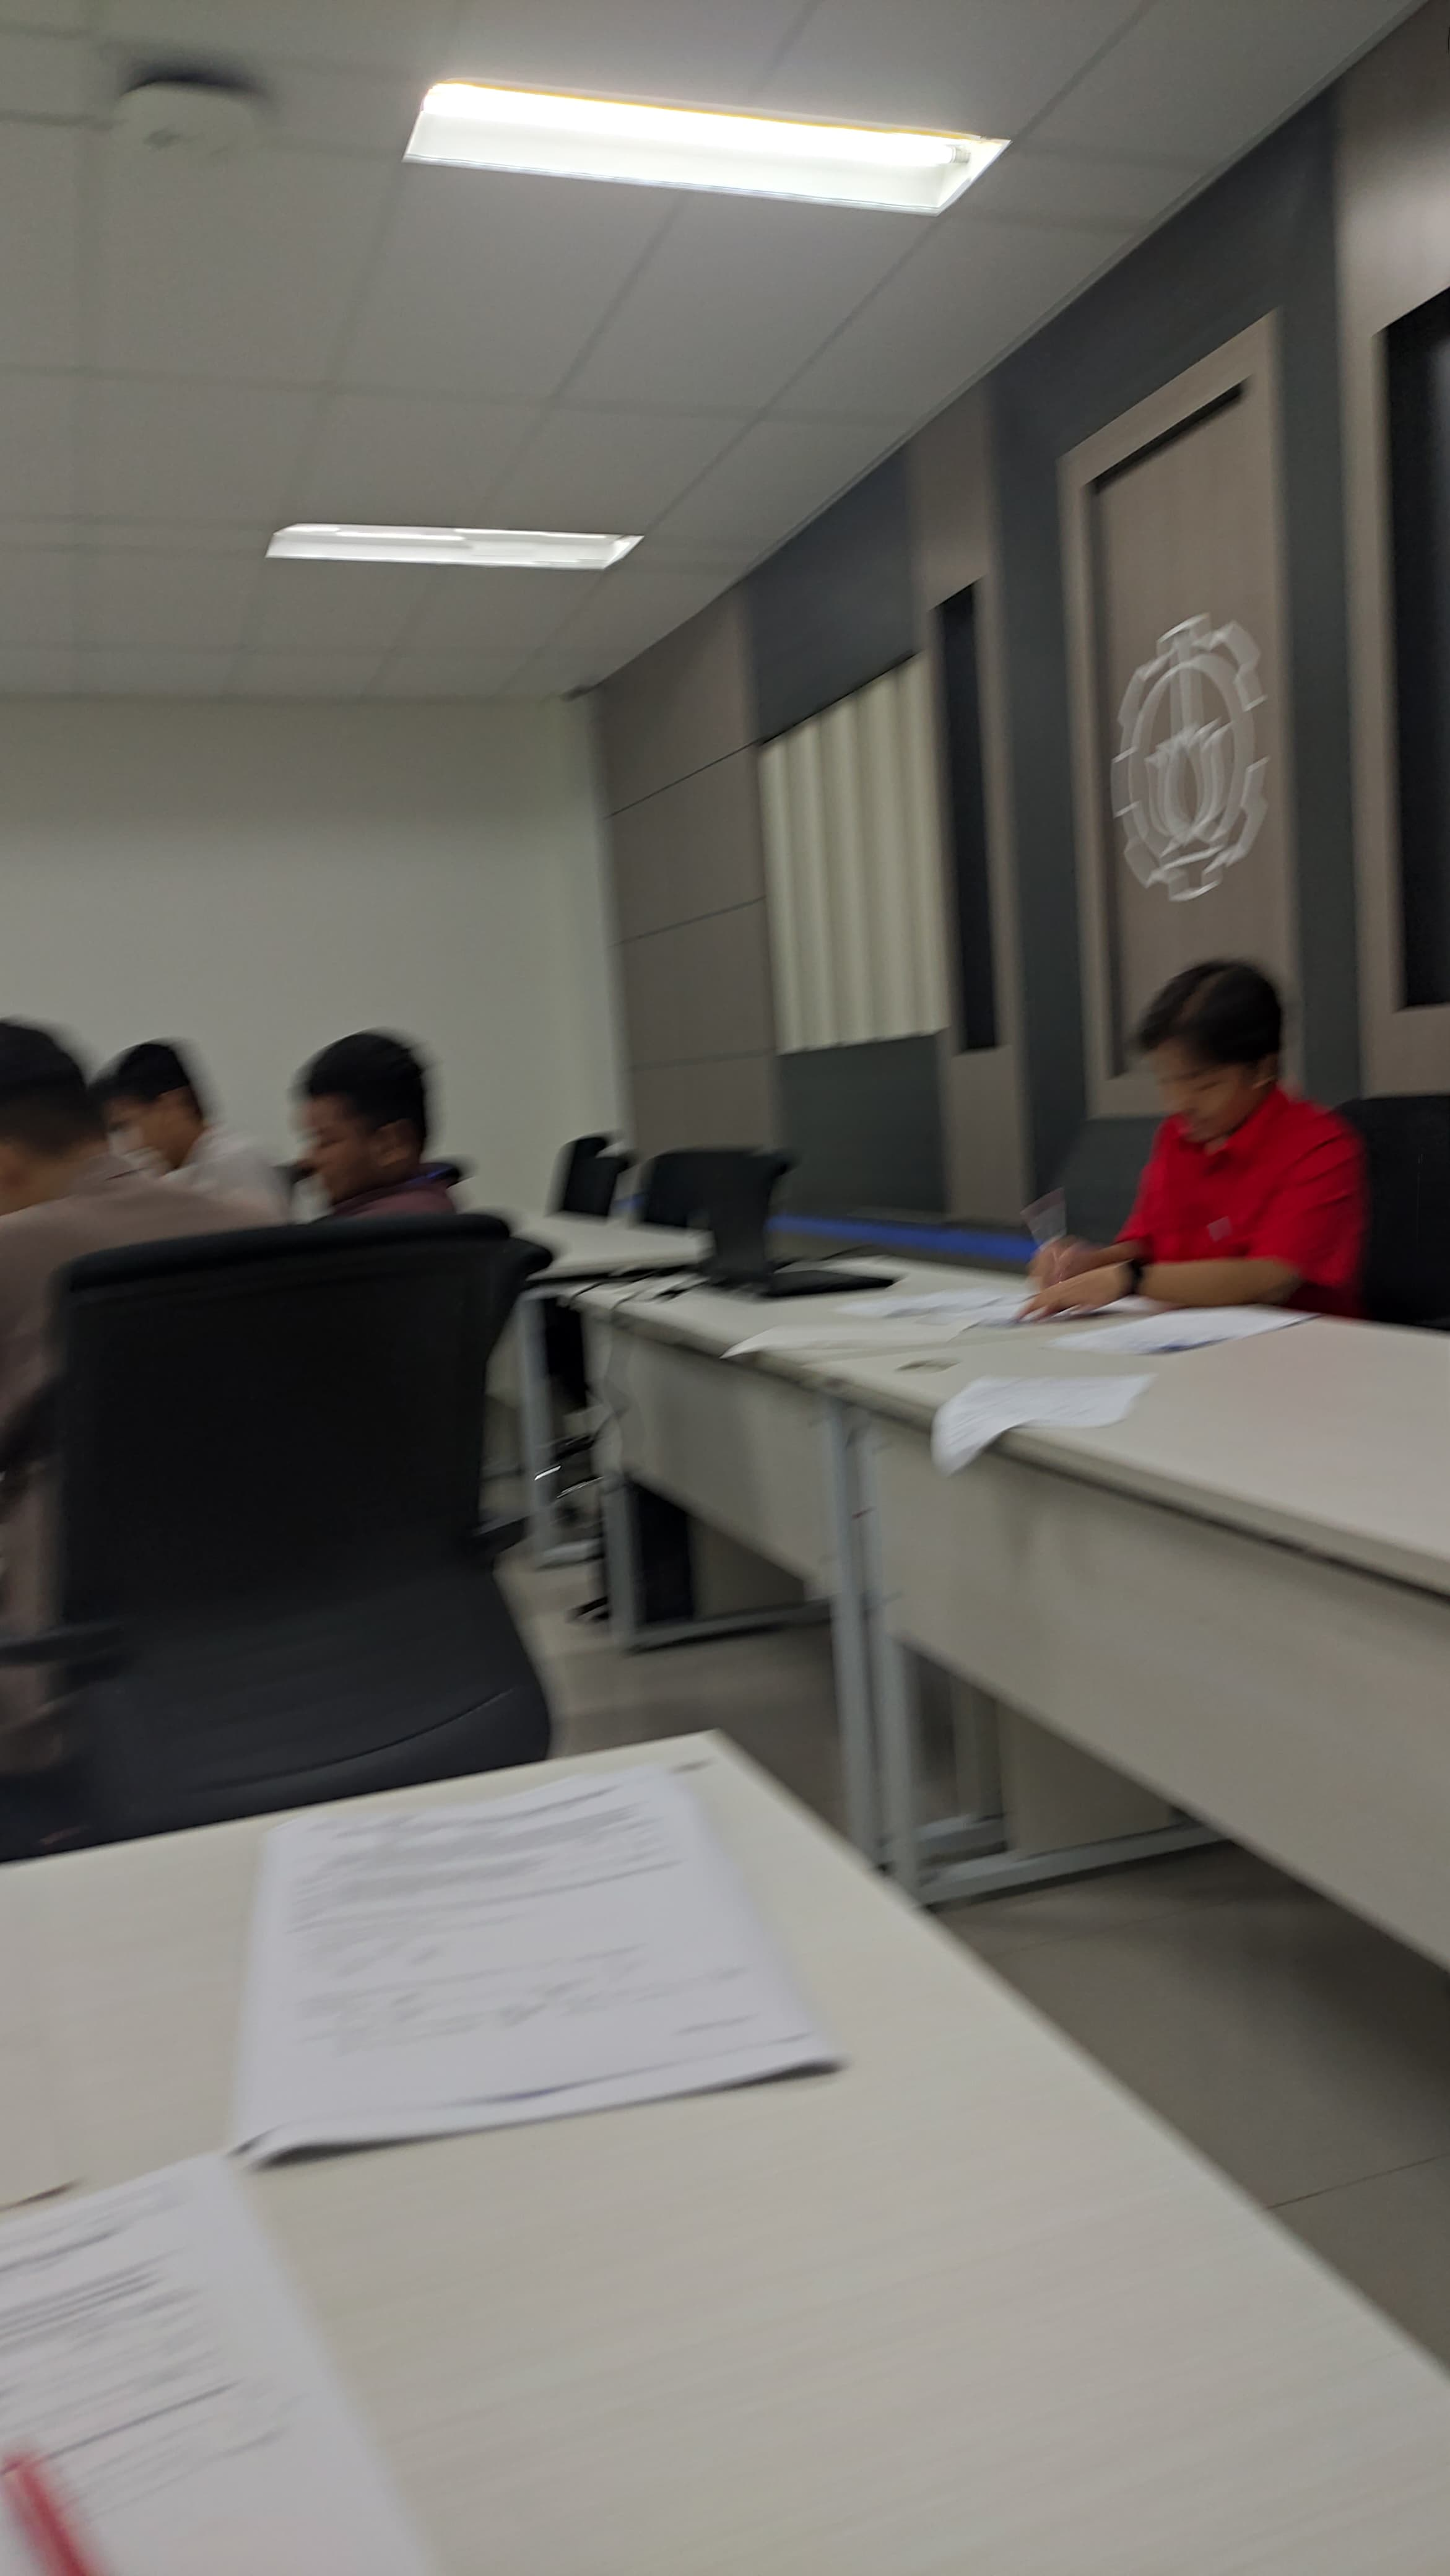
\includegraphics[height=1.6in]{figs/Koreksi4.jpg}
        };
    \end{tikzpicture}
    \begin{tikzpicture}
        \node[draw=black, drop shadow, line width=1pt, inner sep=0] {
          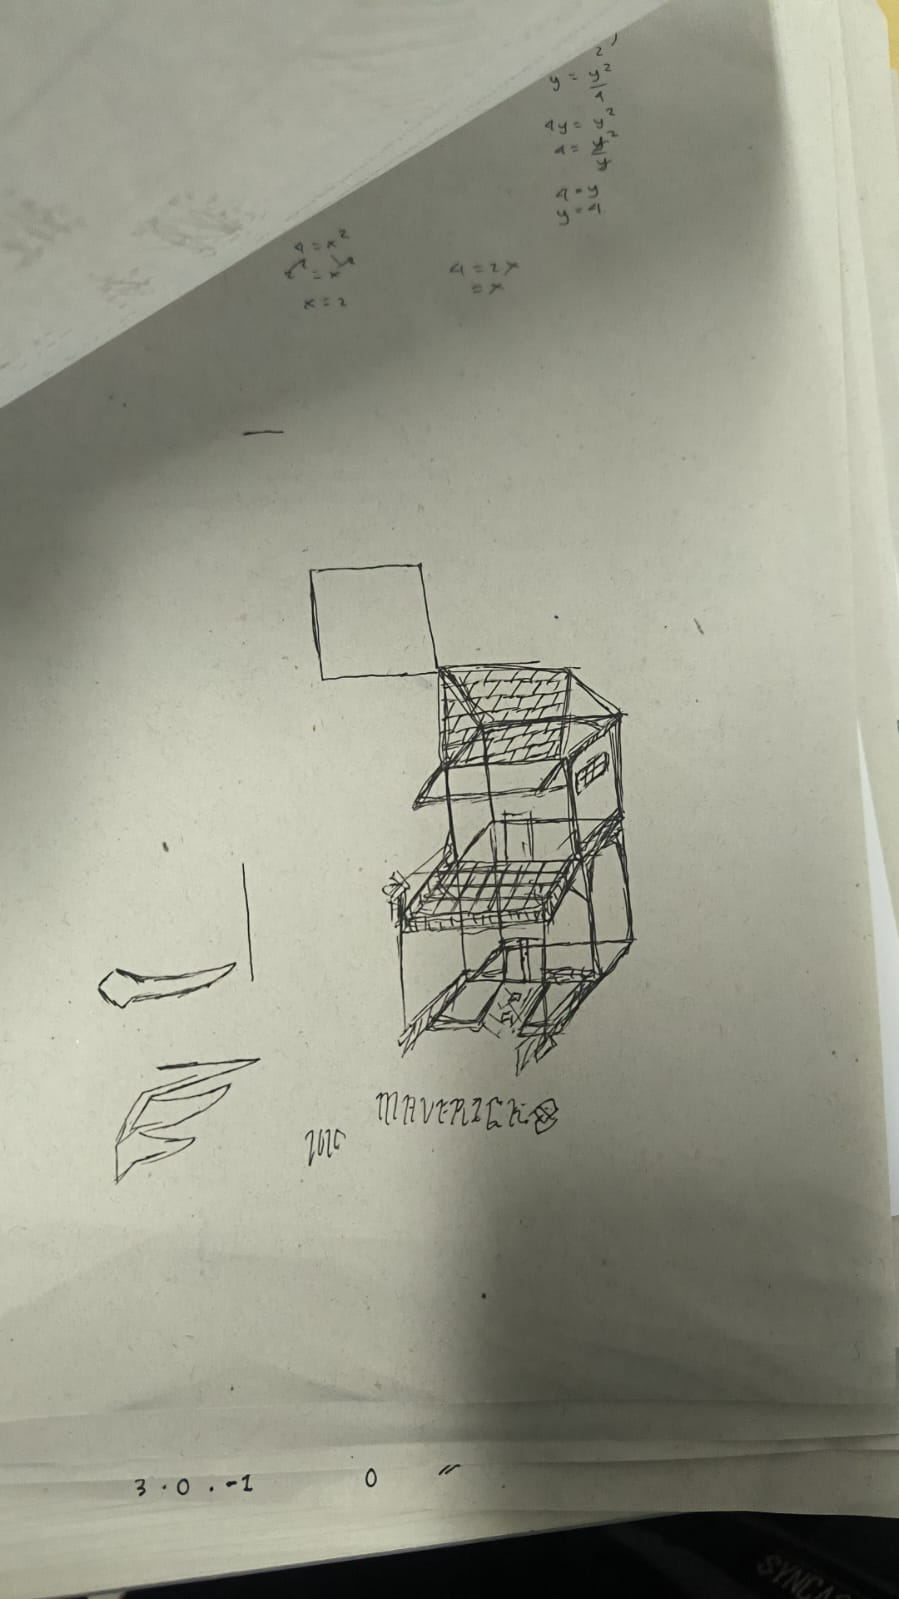
\includegraphics[height=1.6in]{figs/Koreksi5.jpg}
        };
    \end{tikzpicture}
    \caption{Mengoreksi remidial mahasiswa ulang} 
    \end{figure}
    \vfill
\end{frame}

\subsection{Dokumentasi Bersama Rekan}
\begin{frame}
    \frametitle{\insertsubsection}
    \begin{figure}[h]
        \centering
        \begin{subfigure}[t]{0.3\textwidth}
            \centering
            \begin{tikzpicture}
                \node[draw=black, drop shadow, line width=1pt, inner sep=0] {
                  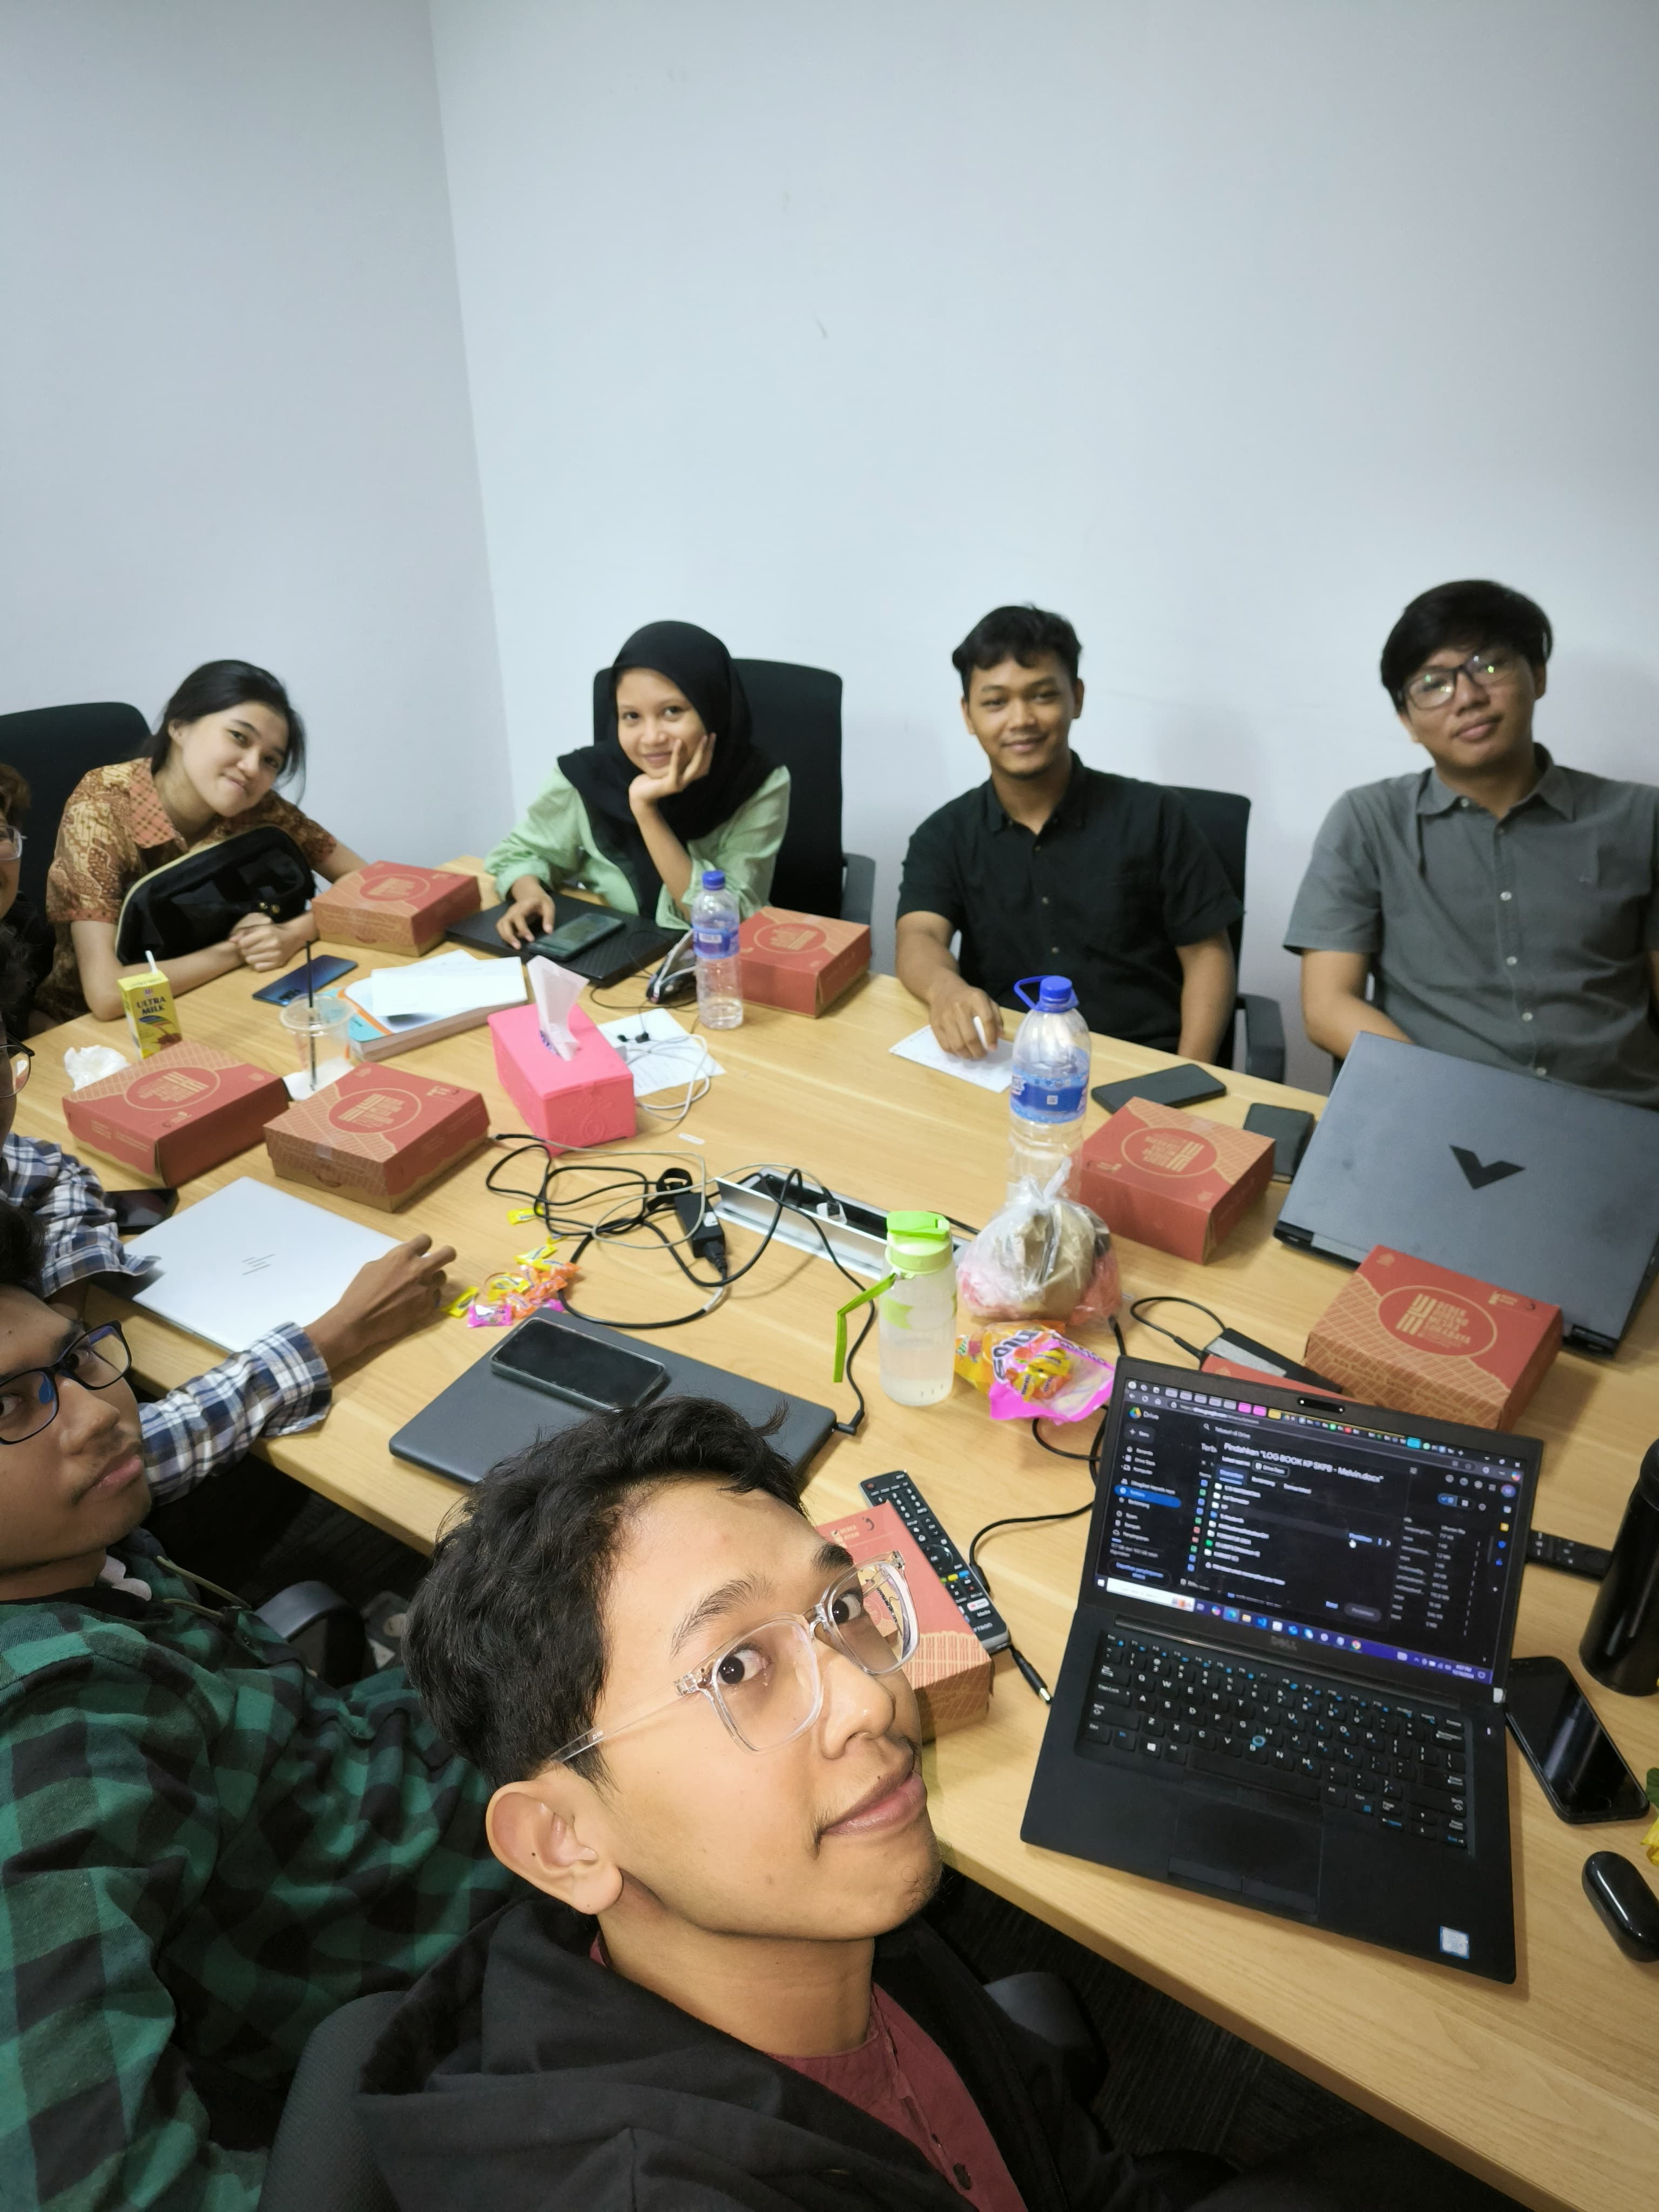
\includegraphics[height=1.7in]{figs/FotbarHabisJaga.jpg}
                };
            \end{tikzpicture}
        \end{subfigure}%
        ~
        \begin{subfigure}[t]{0.3\textwidth}
            \centering
            \begin{tikzpicture}
                \node[draw=black, drop shadow, line width=1pt, inner sep=0] {
                  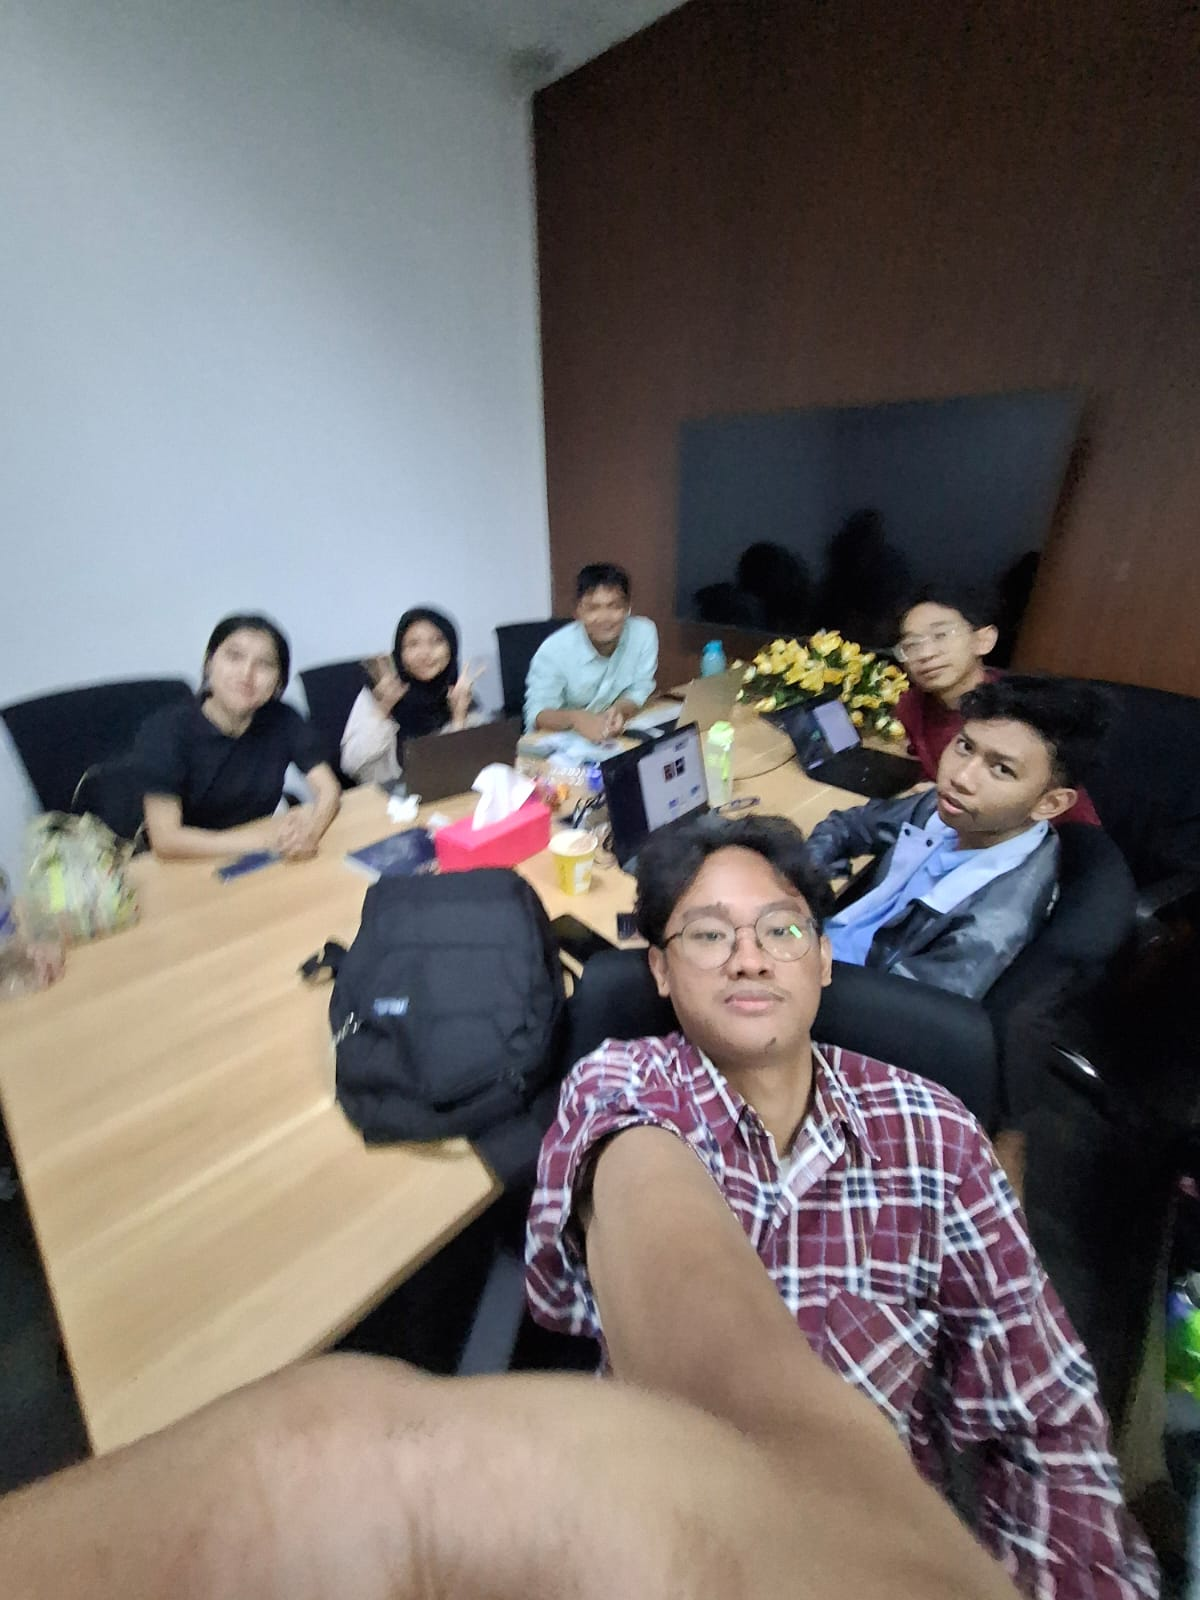
\includegraphics[height=1.7in]{figs/Fotbar2.jpg}
                };
            \end{tikzpicture}
        \end{subfigure}
        ~
        \begin{subfigure}[t]{0.3\textwidth}
            \centering
            \begin{tikzpicture}
                \node[draw=black, drop shadow, line width=1pt, inner sep=0] {
                  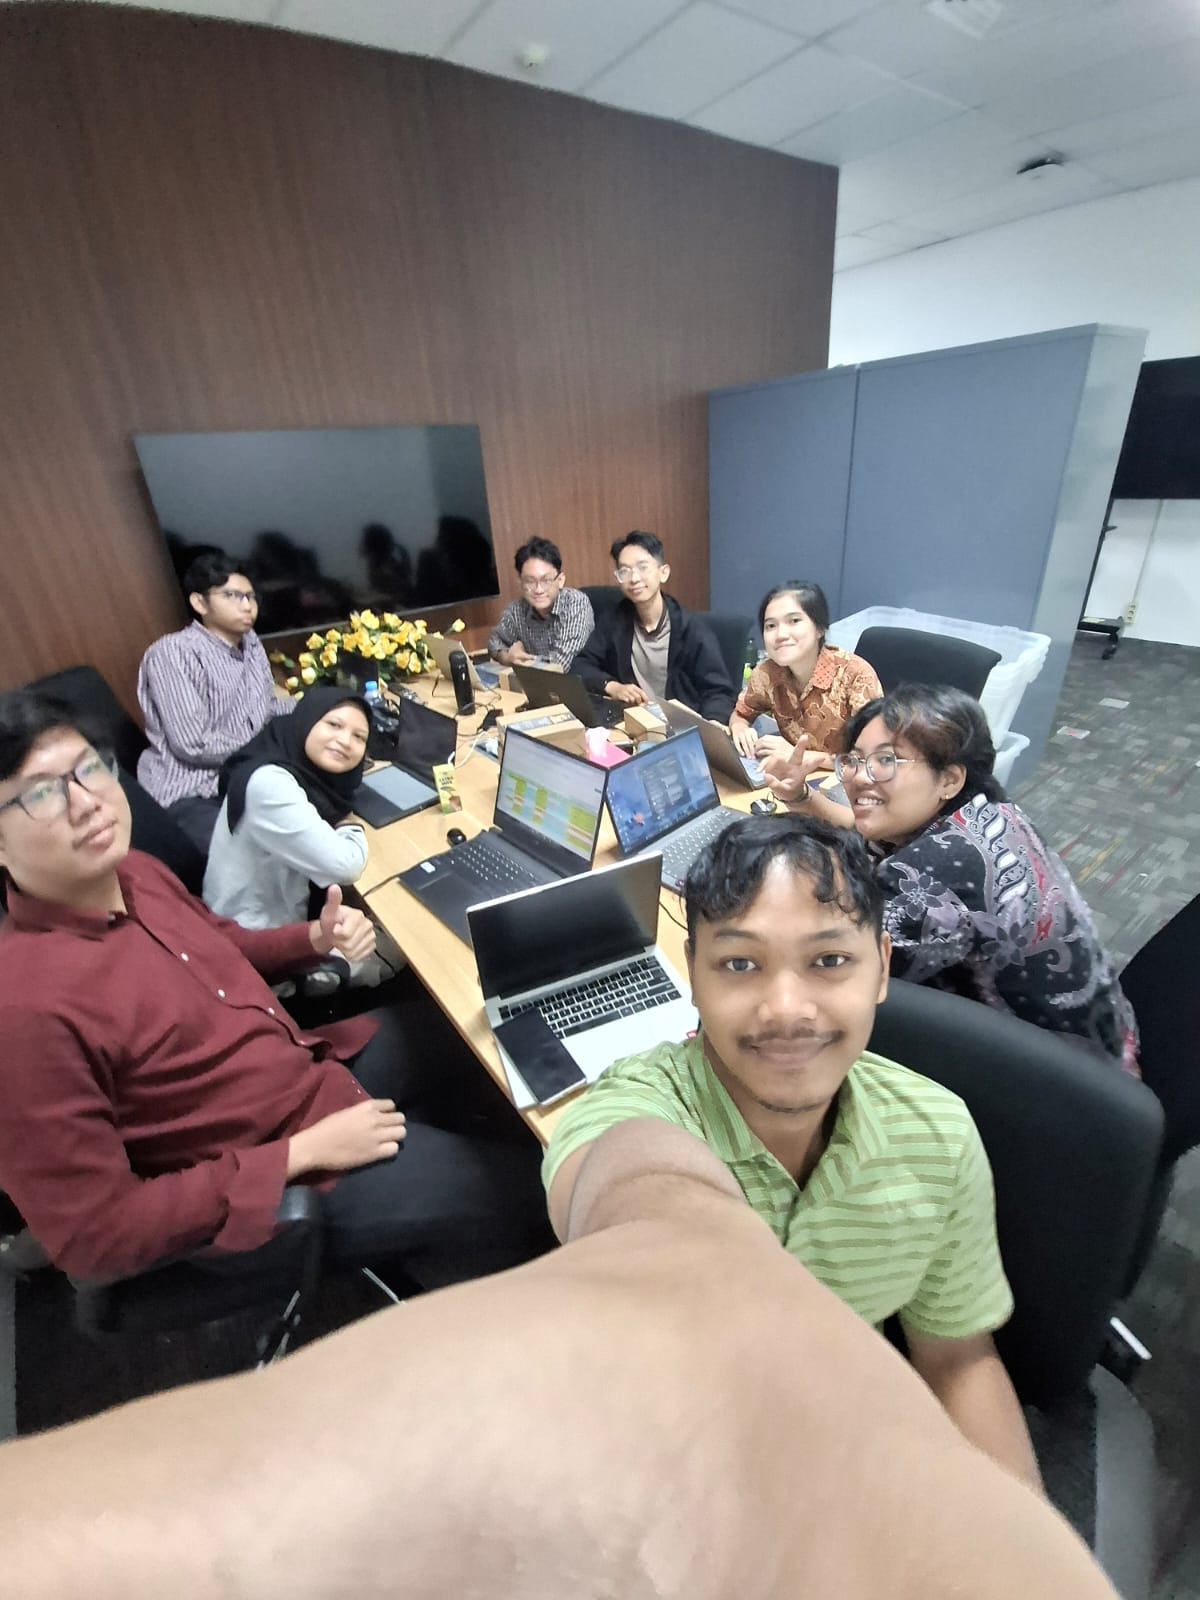
\includegraphics[height=1.7in]{figs/Fotbar1.jpg}
                };
            \end{tikzpicture}
        \end{subfigure}
    \end{figure}
\end{frame}

\begin{frame}
    \vfill
    \begin{figure}[h]
        \begin{subfigure}[t]{0.4\textwidth}
            \centering
            \begin{tikzpicture}
                \node[draw=black, drop shadow, line width=1pt, inner sep=0] {
                  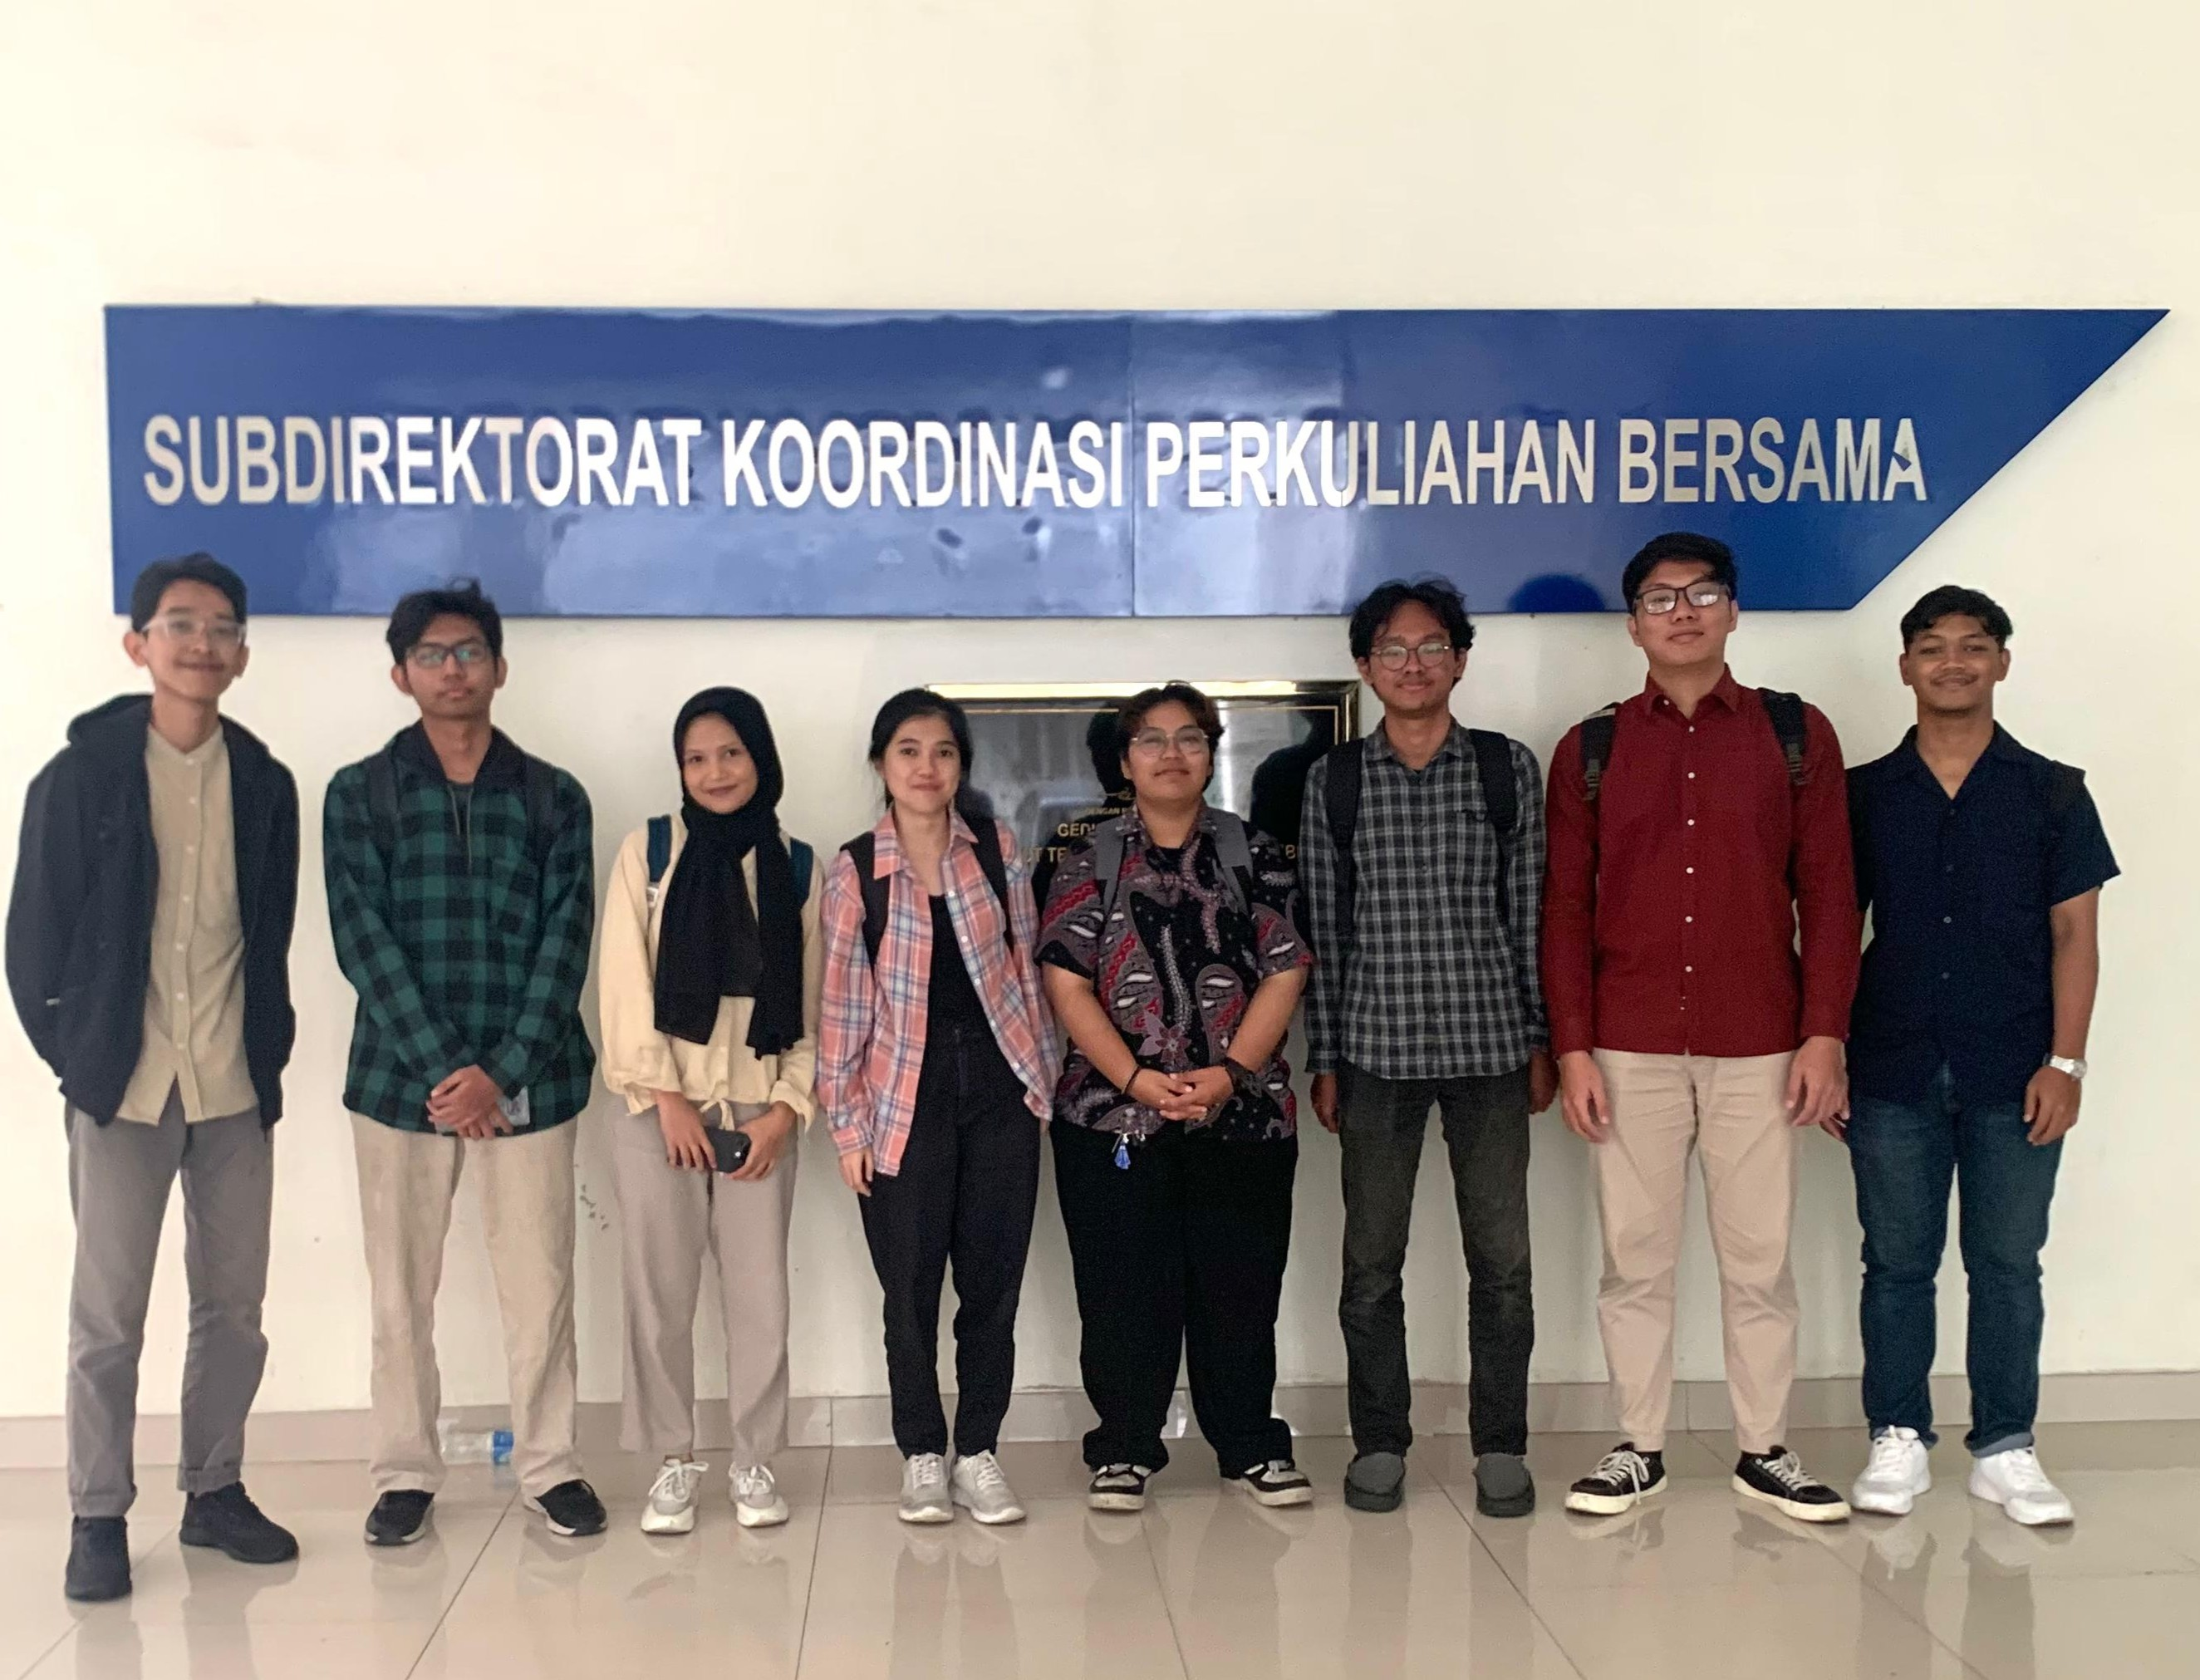
\includegraphics[height=1.7in]{figs/FotbarSKPBLantaiG.jpg}
                };
            \end{tikzpicture}
        \end{subfigure}
        ~\qquad\qquad~
        \begin{subfigure}[t]{0.4\textwidth}
            \centering
            \begin{tikzpicture}
                \node[draw=black, drop shadow, line width=1pt, inner sep=0] {
                  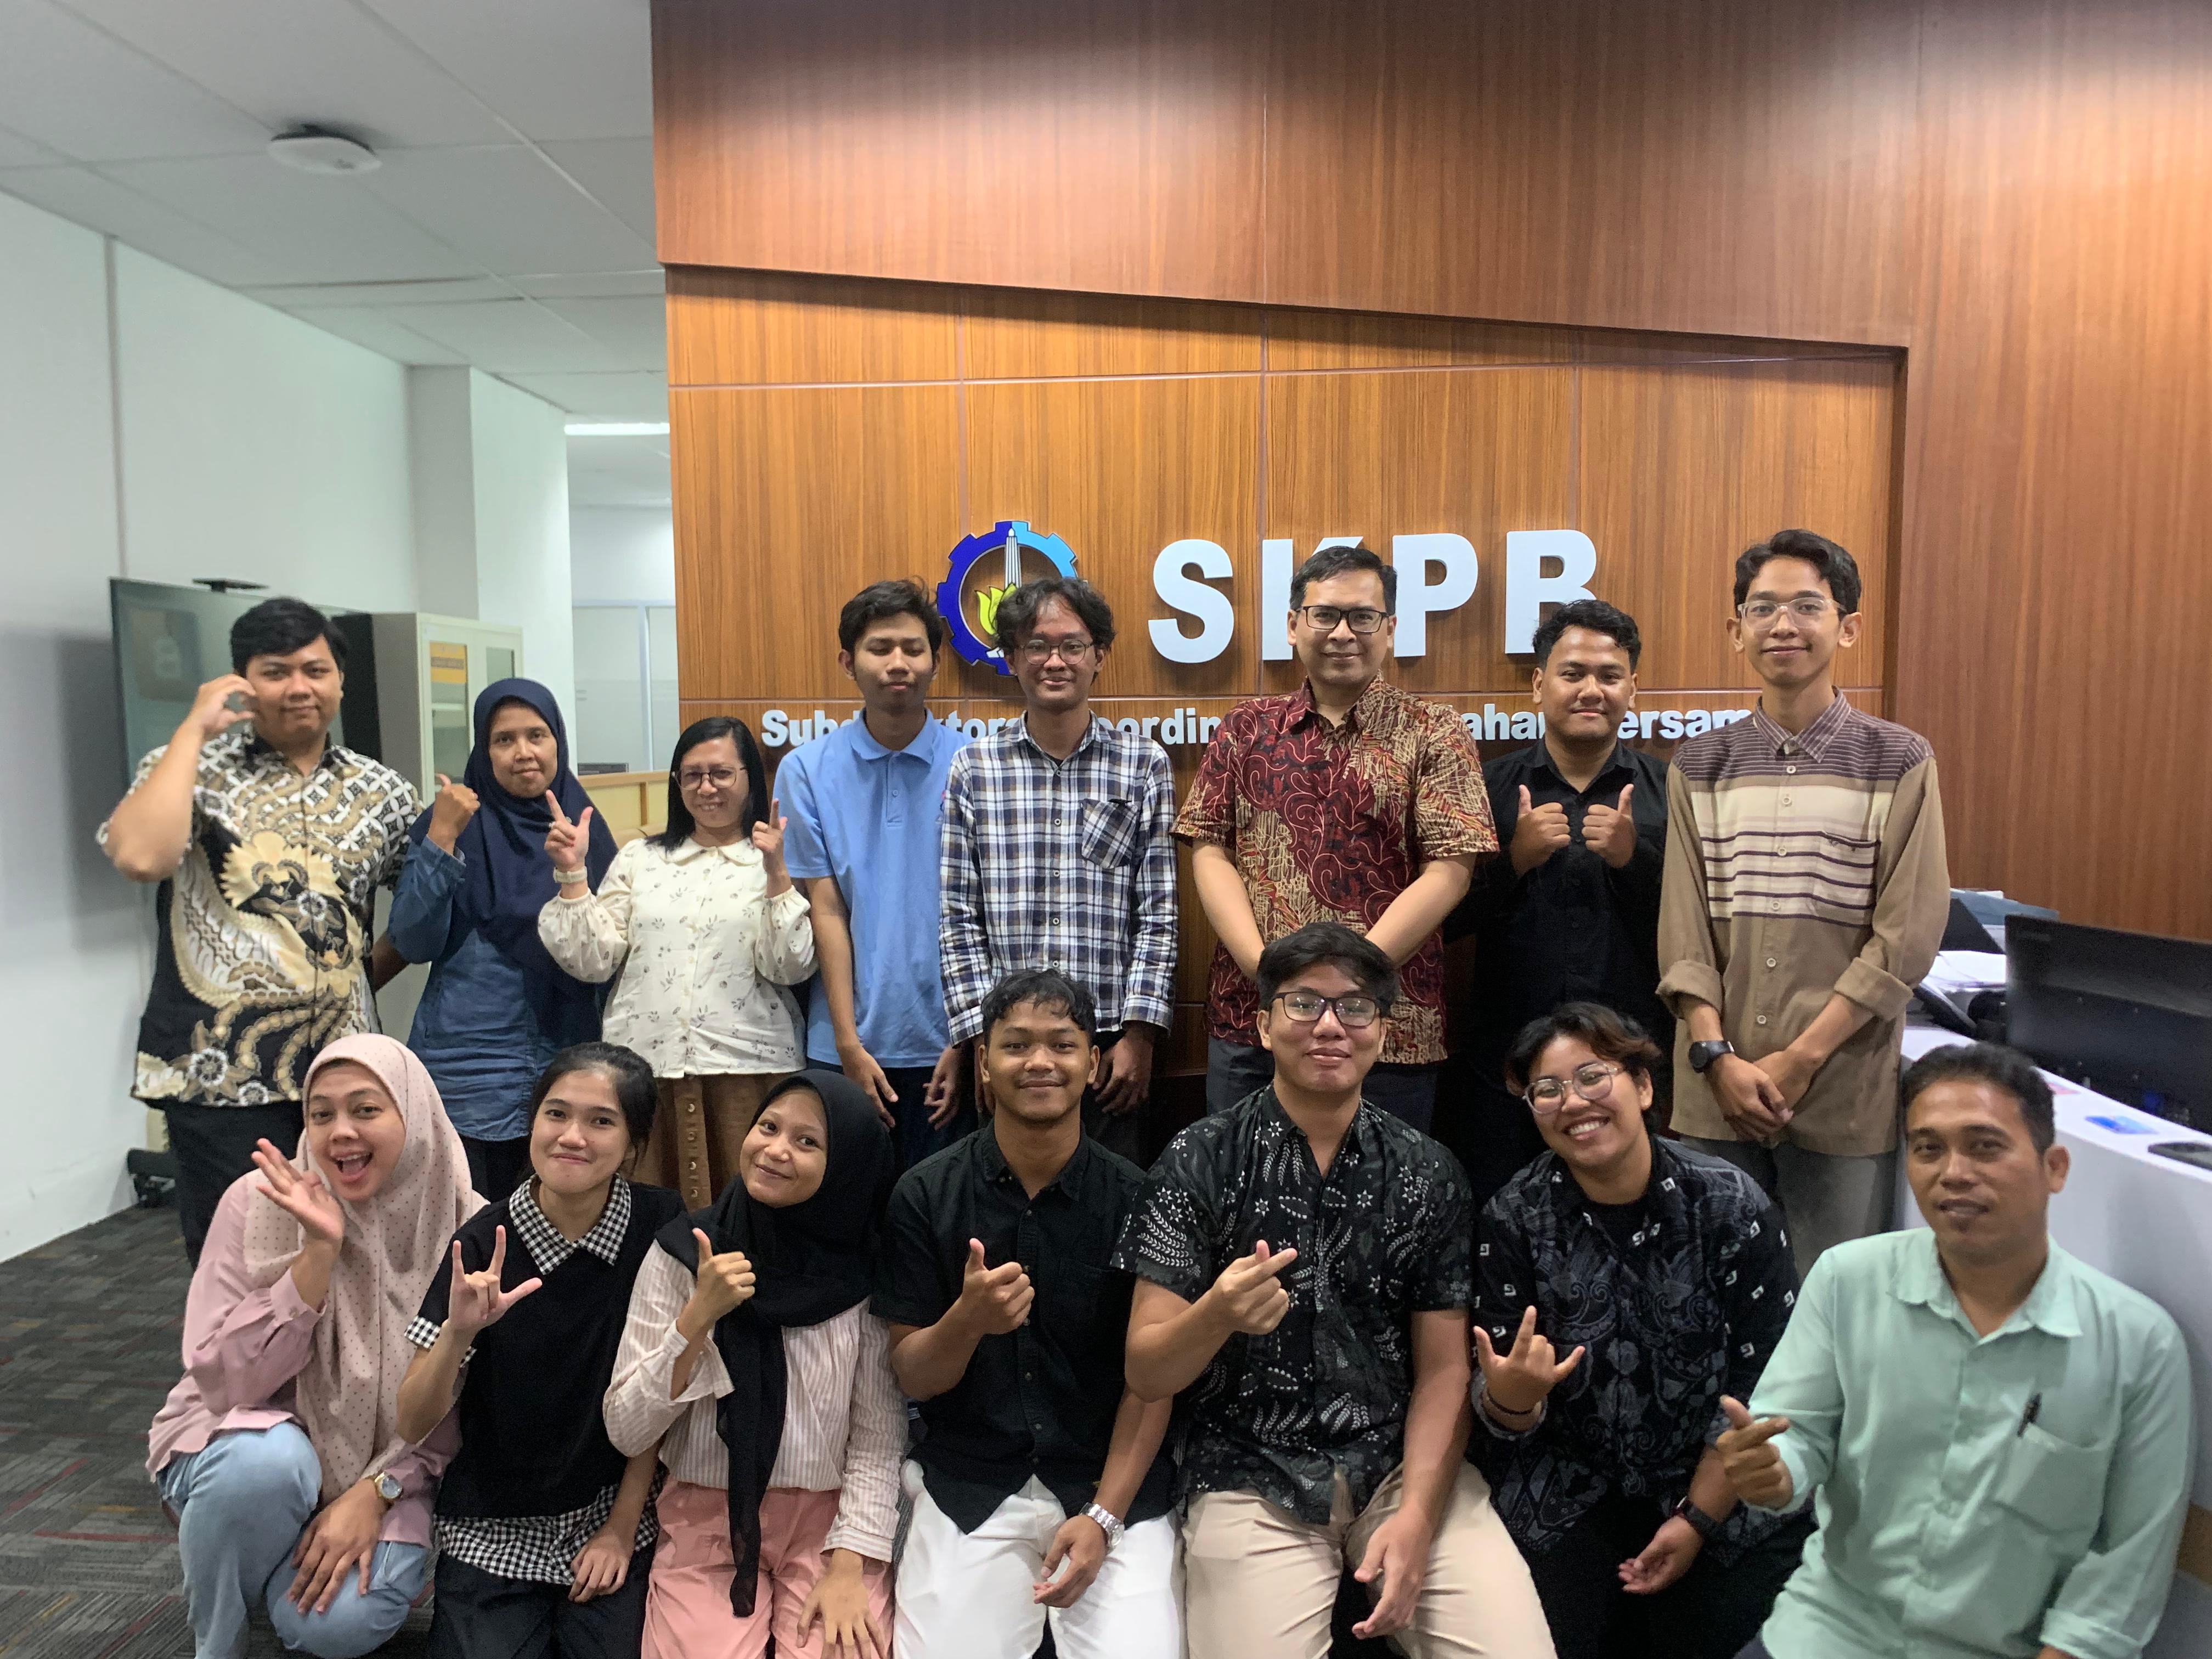
\includegraphics[height=1.7in]{figs/FotbarLobby.jpg}
                };
            \end{tikzpicture}
        \end{subfigure}
    \end{figure}
    \vfill
\end{frame}

\section{Hasil Kerja Praktik}

\setLayout{vertical}
\begin{frame}
    \textit{Source code}: \alert{\underline{\texttt{\href{https://github.com/KP-SKPB/KP-SKPB.github.io}{github.com/KP-SKPB/KP-SKPB.github.io}}}}
    \begin{figure}[h]
        \centering
        \begin{tikzpicture}
            \node[draw=black, drop shadow, line width=1pt, inner sep=0] {
              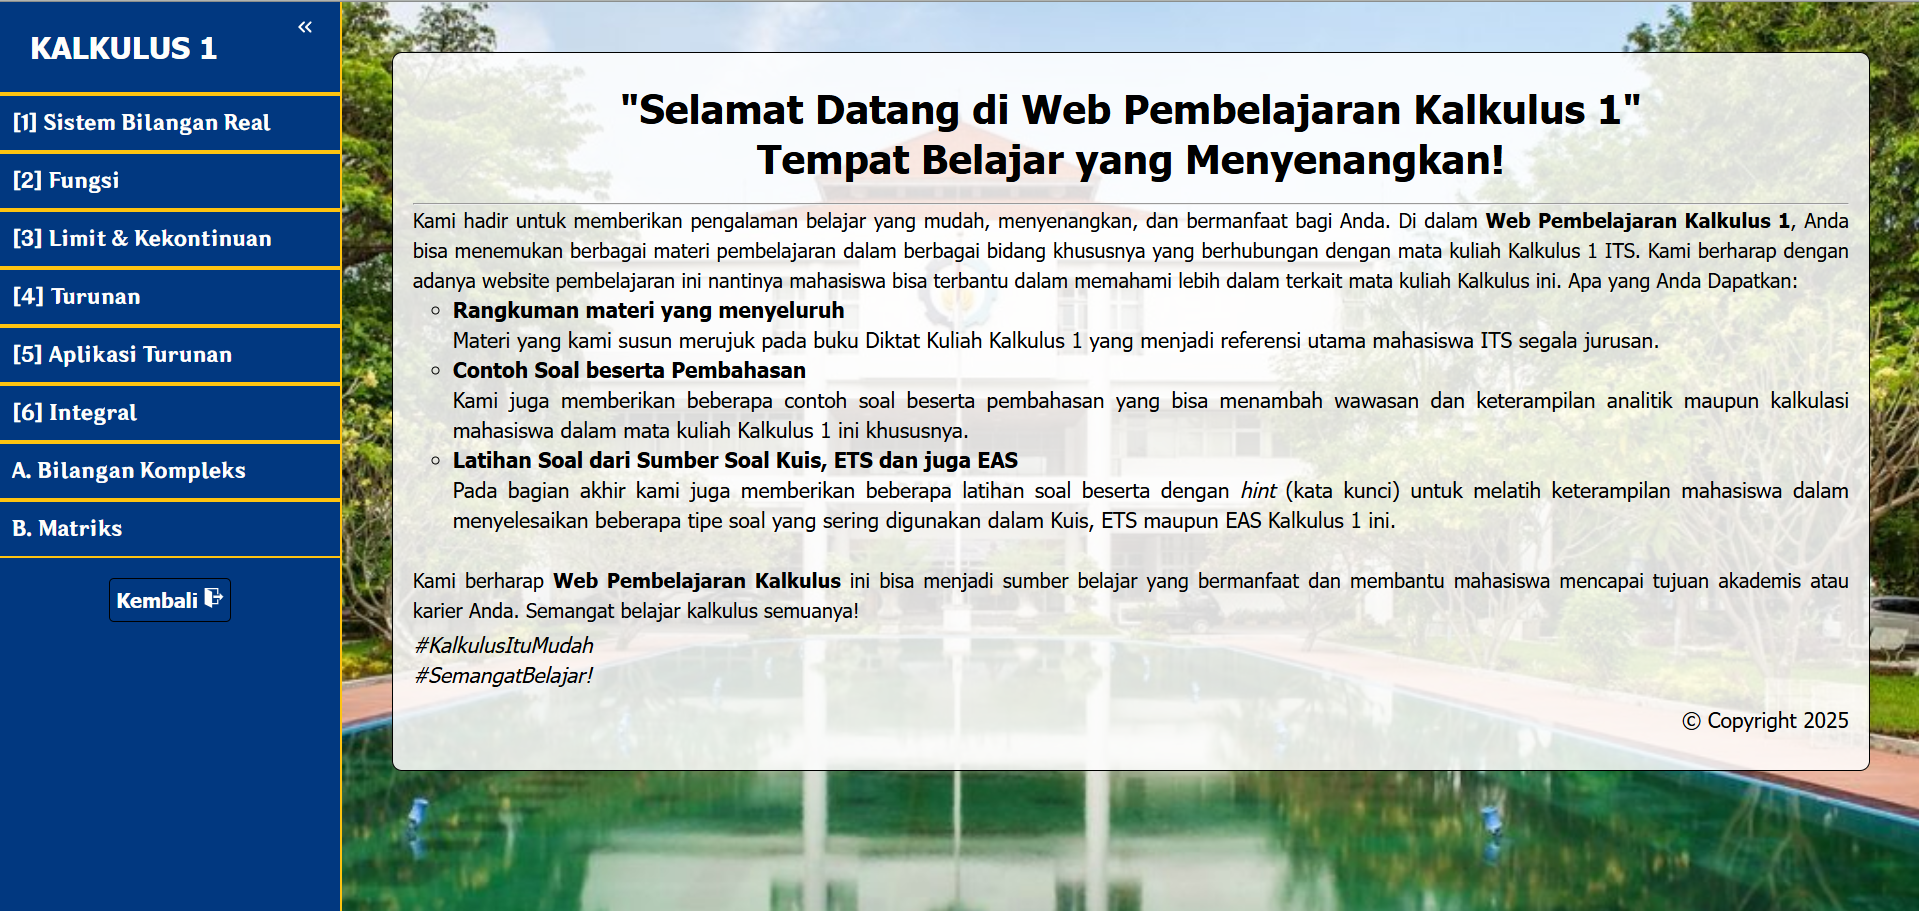
\includegraphics[width=0.55\textwidth]{figs/Hasil1.png}
            };
        \end{tikzpicture}\\~\\
        \begin{tikzpicture}
            \node[draw=black, drop shadow, line width=1pt, inner sep=0] {
              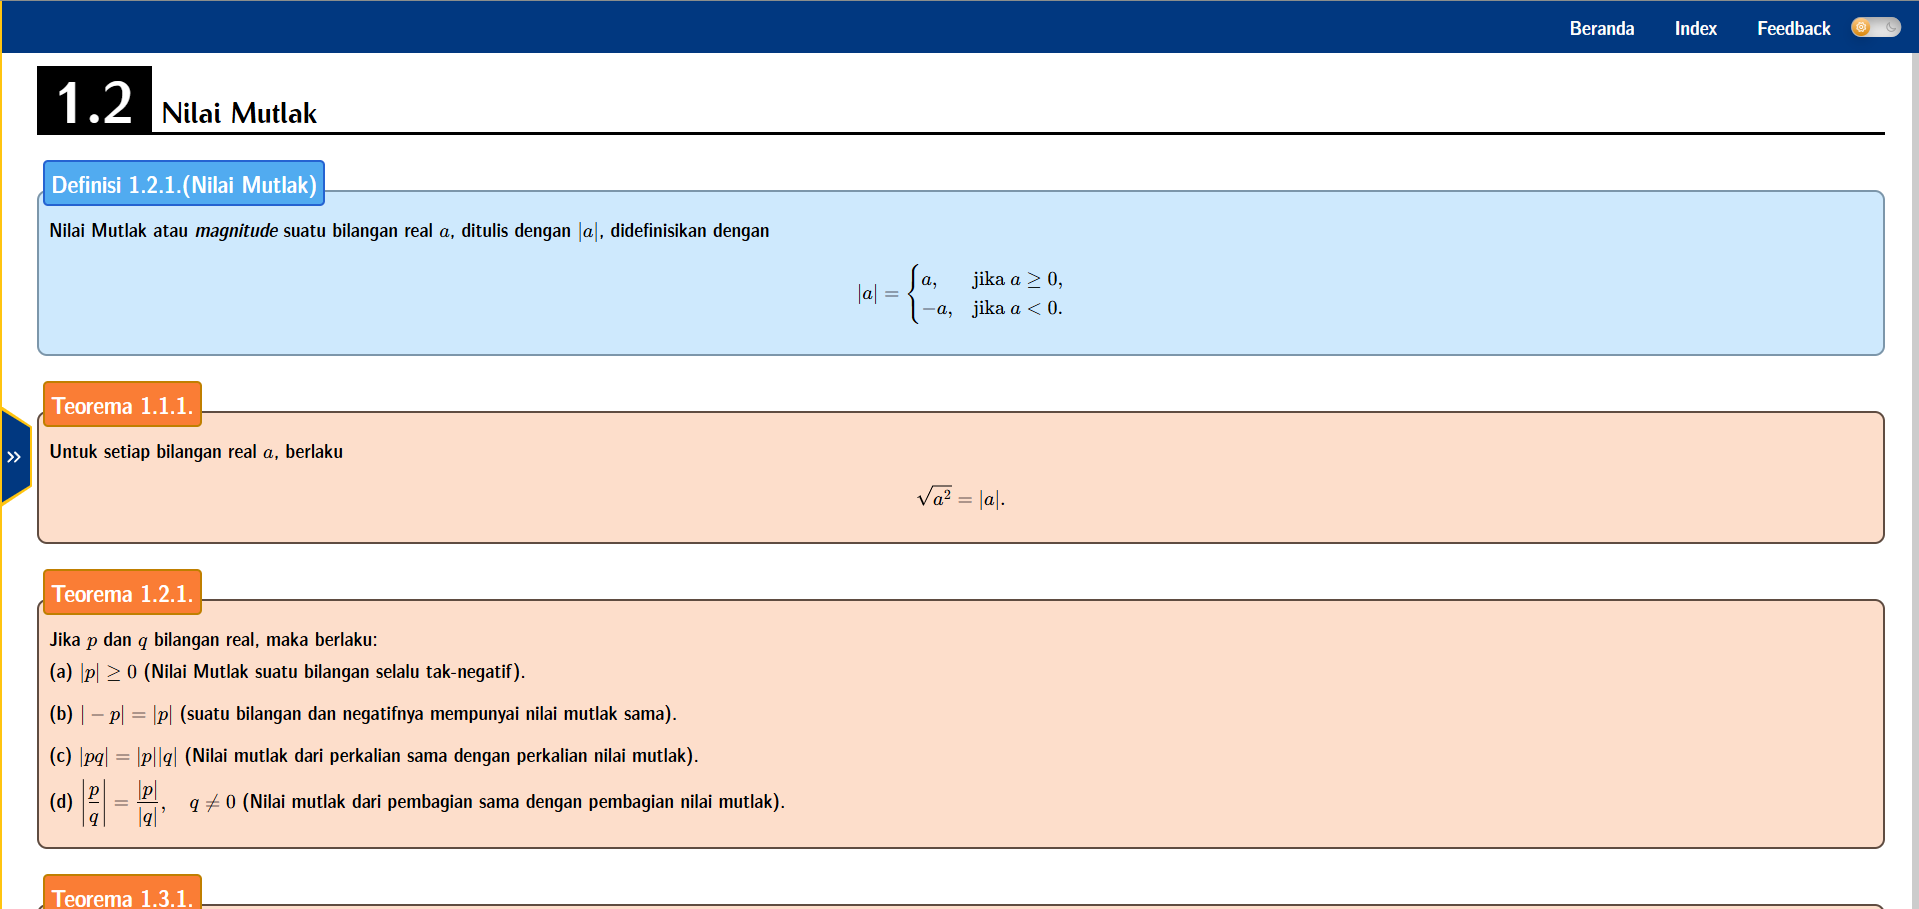
\includegraphics[width=0.55\textwidth]{figs/Hasil2.png}
            };
        \end{tikzpicture}
    \end{figure}
\end{frame}

\begin{frame}
    \textit{Source code}: \alert{\underline{\texttt{\href{https://github.com/KP-SKPB/KP-SKPB.github.io}{github.com/KP-SKPB/KP-SKPB.github.io}}}}
    \begin{figure}[h]
        \centering
        \begin{tikzpicture}
            \node[draw=black, drop shadow, line width=1pt, inner sep=0] {
              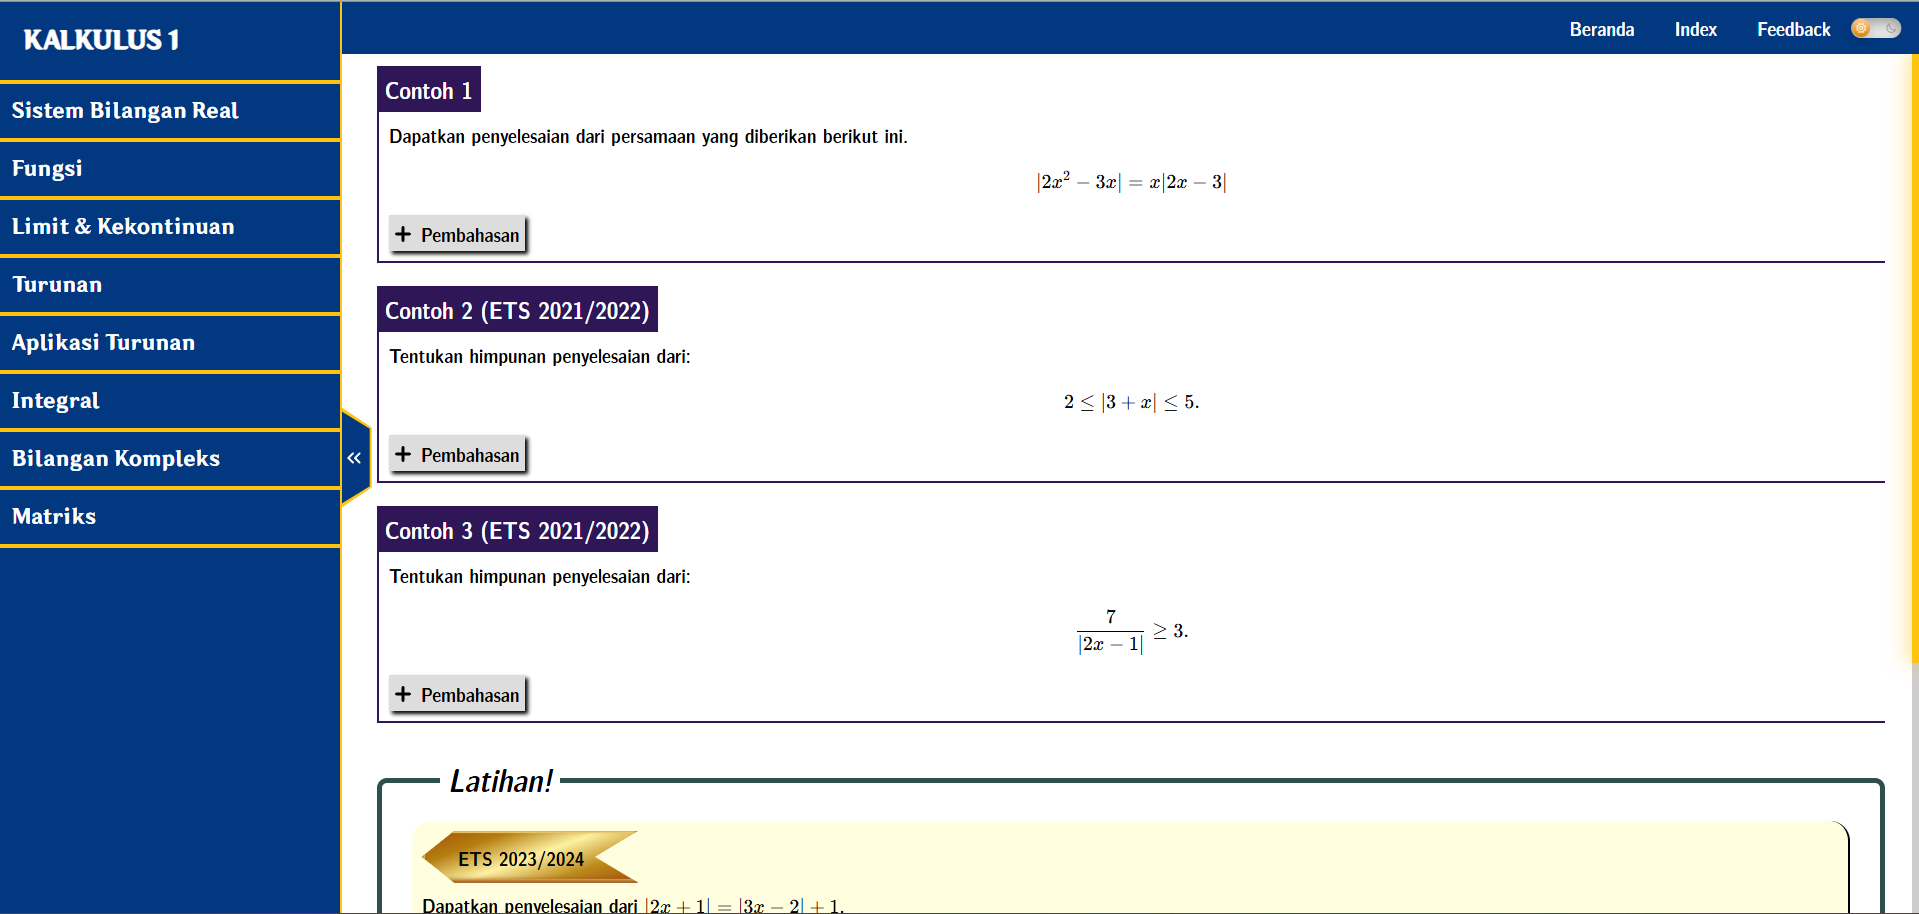
\includegraphics[width=0.55\textwidth]{figs/Hasil3.png}
            };
        \end{tikzpicture}\\~\\
        \begin{tikzpicture}
            \node[draw=black, drop shadow, line width=1pt, inner sep=0] {
              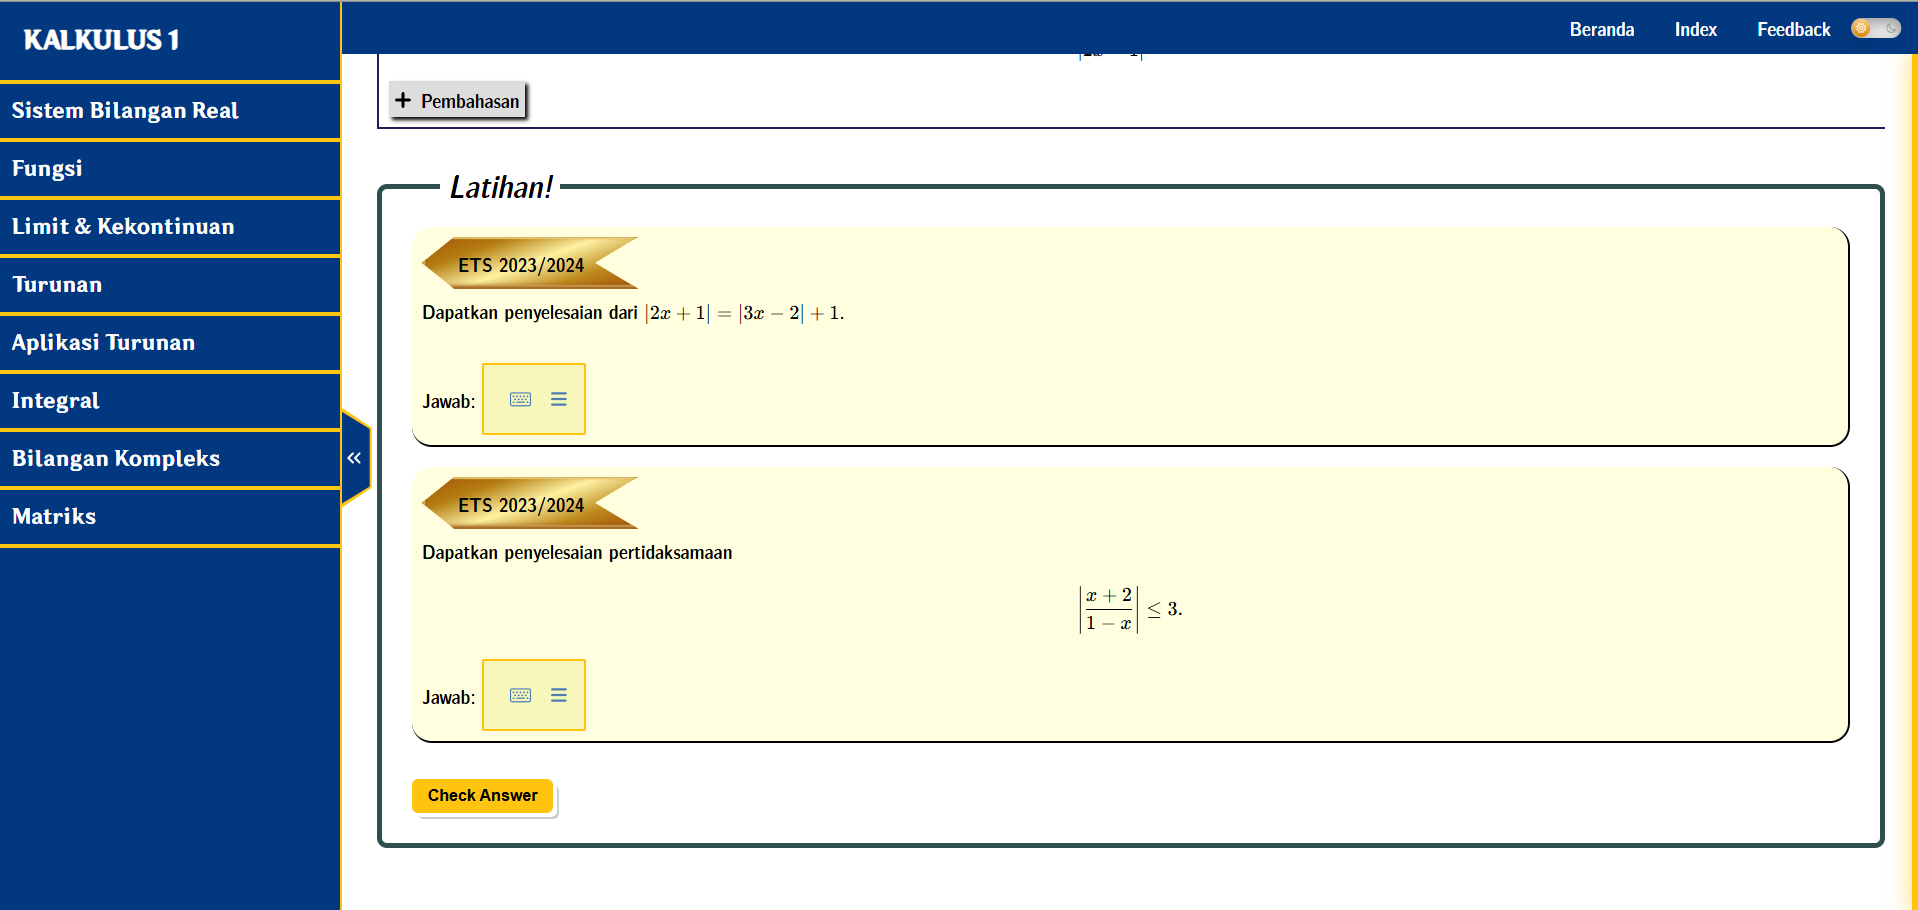
\includegraphics[width=0.55\textwidth]{figs/Hasil4.png}
            };
        \end{tikzpicture}
    \end{figure}
\end{frame}

\section{Penutup: Kesimpulan dan Saran}

\setLayout{horizontal}
\begin{frame}
    \begin{columns}
        \column{0.5\textwidth}
            \begin{block}{Kesimpulan}
                \begin{itemize}
                    \item Kerja praktik di SKPB memberikan pengalaman berharga dalam pembuatan website.
                    \item Website kalkulus diharapkan membantu mahasiswa dalam memahami materi kalkulus.
                    \item \textit{CortexJS} dapat digunakan untuk fleksibilitas jawaban pengguna.
                \end{itemize}
            \end{block}
        \column{0.5\textwidth}
            \begin{block}{Saran}
                \begin{itemize}
                    \item Perlu adanya pengembangan lebih lanjut pada website kalkulus.
                    \item Disarankan untuk melakukan uji coba lebih banyak dengan mahasiswa untuk mendapatkan umpan balik.
                    \item Perlu penambahan fitur responsif pada versi mobile.
                \end{itemize}
            \end{block}
    \end{columns}
\end{frame}


%---------------------------------------------------------

\setLayout{thankyou}
\begin{frame}
    
    \centering
    \vspace{2cm}
    
    \textbf{\Huge Terima Kasih}
    
    \ \\
    
    \textbf{Website hasil kerja praktik dapat diakses melalui link berikut:}
    \ \\

    \text{\ttfamily\color{blue} \underline{\href{https://kp-skpb.github.io/Kalkulus\%201/}{kp-skpb.github.io/Kalkulus\%201/}}}
    \vspace{2cm}
    \begin{figure}
        \centering
        \begin{subfigure}{0.2\textwidth}
            \centering
            \includegraphics[height=1.5cm]{lib/logos/ITSMath.pdf}
        \end{subfigure}
        \qquad
        \begin{subfigure}{0.2\textwidth}
            \centering
            
\includegraphics[height=1.2cm]{lib/logos/LogoPerusahaan.png}
        \end{subfigure}
    
    \end{figure}

\end{frame}
%---------------------------------------------------------Slide 9


\end{document}